\chapter{Experiments\&Results}

\section{Datasets}

We evalute our models on three different datasets.
The dataset size is primarily limited by the computational resources, such as memory and computation time. 

\subsection{1x4 Dataset}

The simplest dataset we use a 1 dimensional binary dataset of size 4, where either the first or the last element is set to 1. 

\begin{figure}[h!]
	\centering
    	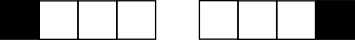
\includegraphics[width=0.7\textwidth]{imgs/1x4_ds.png} 
    \caption{The two samples of the 1x4 dataset.}
	\label{fig:test}
\end{figure}

\subsection{Stripe Dataset}

We generate a $10 \times 10$ pixel noisy stripe dataset, with three different oriented stripes, horizontal, diagonal, vertical. 
This could represent a similar object to a pen recorded with a event-based camera, and result in an grasp id.
In the easiest version of this dataset, the stripes always occur on the same places, with some random noise.
An more complex version of the datasets contains the stripes randomly distributed across the whole image.
The dataset can be either binary or continuous.


\begin{figure}[h!]
	\centering
	\begin{subfigure}[t]{.49\textwidth}
  		\centering
  		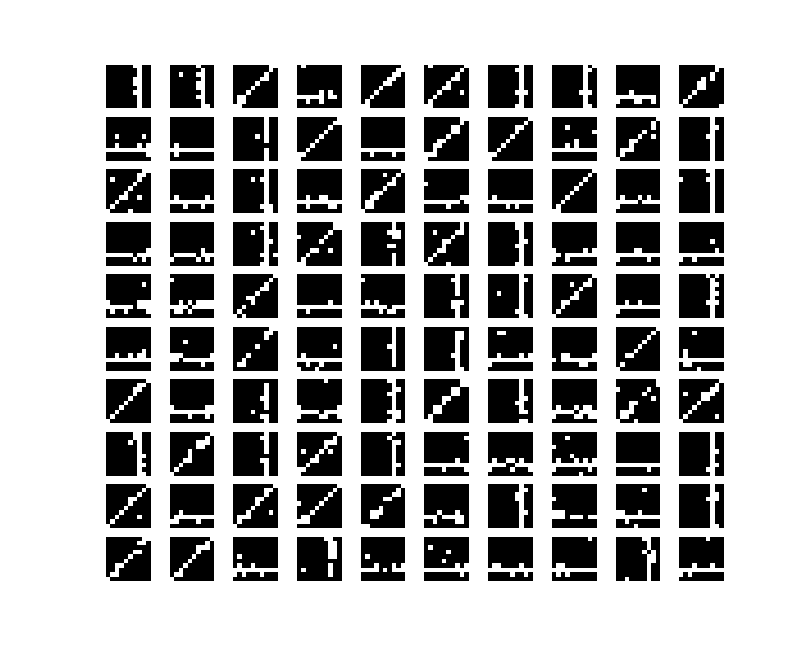
\includegraphics[width=.9\linewidth]{imgs/stripes1.png}
  		\caption{Samples from the unshifted binary stripe dataset.}
  		\label{fig:sub1}
	\end{subfigure}%
	\begin{subfigure}[t]{.49\textwidth}
  		\centering
  		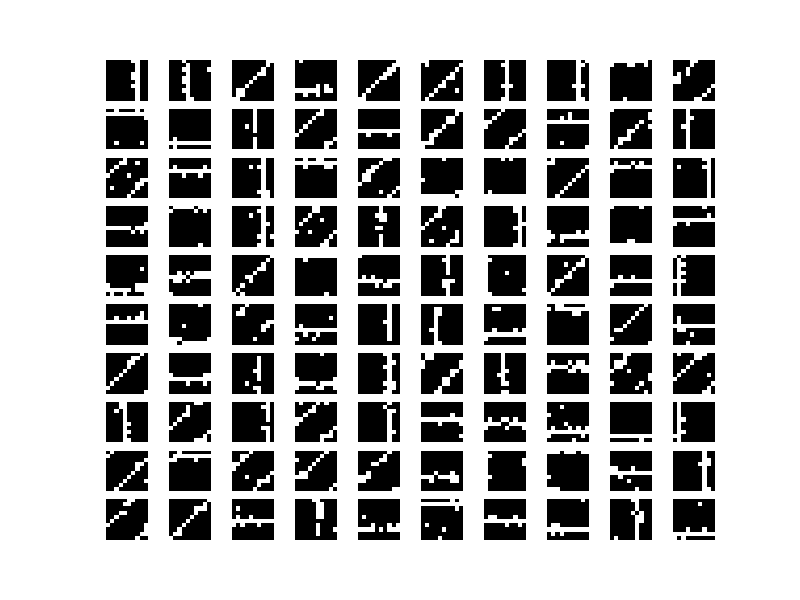
\includegraphics[width=.9\linewidth]{imgs/stripes2.png}
  		\caption{Samples from the  shifted binary stripe dataset.}
  		\label{fig:sub2}
	\end{subfigure}
	\begin{subfigure}[t]{.49\textwidth}
  		\centering
  		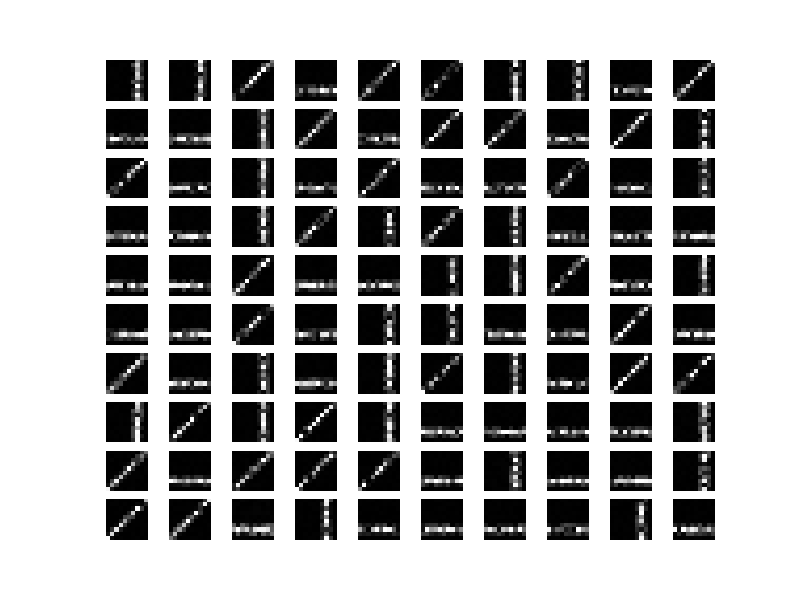
\includegraphics[width=.9\linewidth]{imgs/stripes3.png}
  		\caption{Samples from the unshifted continuous stripe dataset.}
  		\label{fig:sub2}
	\end{subfigure}
	\begin{subfigure}[t]{.49\textwidth}
  		\centering
  		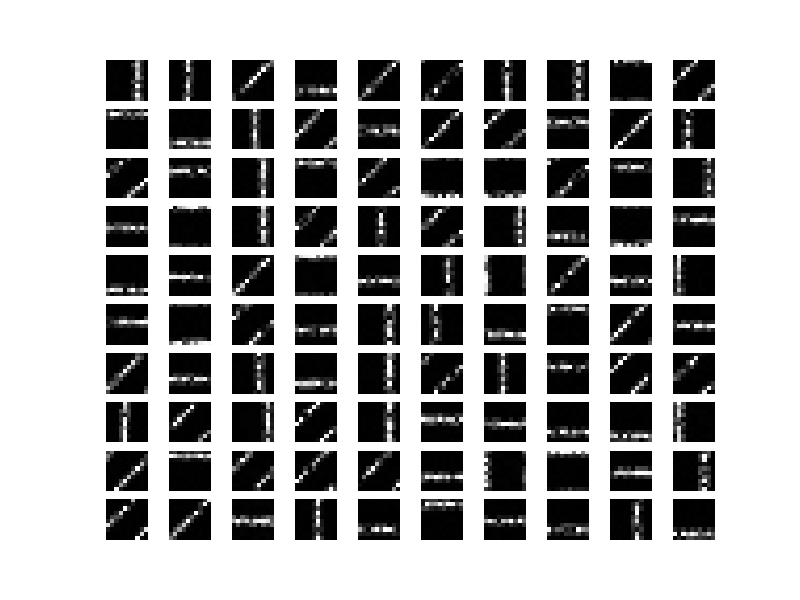
\includegraphics[width=.9\linewidth]{imgs/stripes4.png}
  		\caption{Samples from the shifted continuous stripe dataset.}
  		\label{fig:sub2}
	\end{subfigure}
	\caption{Samples from the stripe dataset. }
	\label{fig:stripes}
\end{figure}


\subsection{MNIST}

We also evaluate the models on the MNIST dataset. 
The MNIST dataset consists of 60000 28x28 pixel gray images of handwritten numbers 0-9.
We evaluate our models on the normal MNIST dataset, as well as a to dvs events converted version of MNIST.

\begin{figure}[h!]
	\centering
    	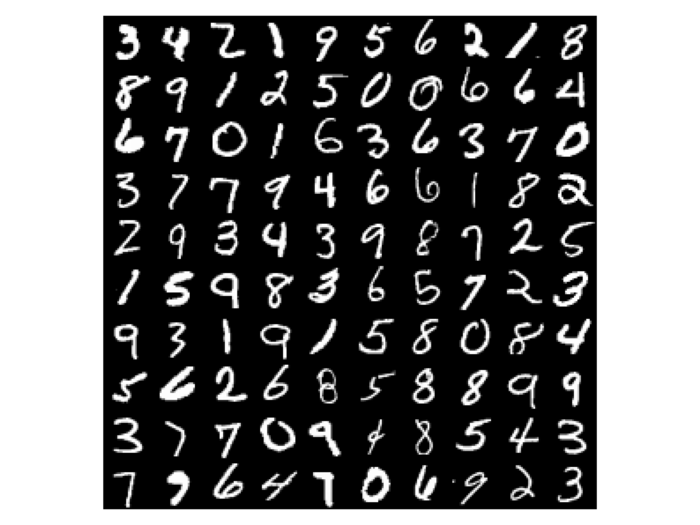
\includegraphics[width=0.7\textwidth]{imgs/mnist.png} 
    \caption{Samples from the MNIST dataset.}
	\label{fig:mnist}
\end{figure}


\subsection{Poker-DVS}

Another dataset used in this thesis is the Poker DVS dataset.
The Dataset consists of 131 poker pip symbols extracted from 3 separate DVS recordings, while quickly browsing poker cards.
From the $128 \times 128$ recorded image, a $32 \times 32$ pixel patch, containing the symbol is extracted.
As a compromise between computational and classification performance, we down sample the patches to a size of $16 \times 16$ pixels and only consider the first $1000$ spikes, due to the constricted learning time per sample.
The resulting dataset is visualized as a accumulation over time in Fig X.
 
    
\begin{figure}[h!]
	\centering
    	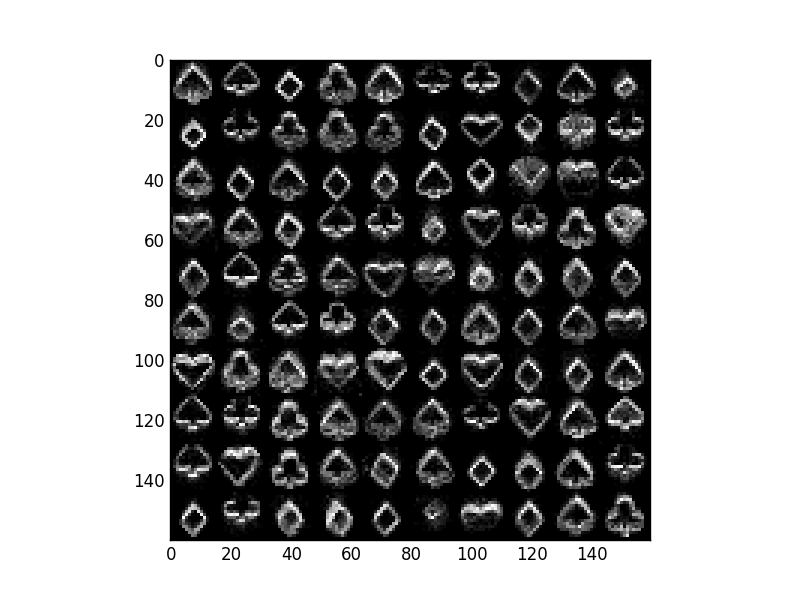
\includegraphics[width=0.7\textwidth]{imgs/poker_ds.png} 
    \caption{Visualization of samples from the Poker-DVS dataset.}
	\label{fig:mnist}
\end{figure}


\section{Experiments}

We orient our experiments primarily on the stripe dataset, due to time and computational constrains which will be explained at first.
After evaluating our models on the stripe dataset, we look on the performance on other datasets for comparison and generalization.     

\subsection{Computational Constrains}

Most of the experiments were executed on a quad-core processor with 3.2 GHz, 16 GB RAM and a NVidia GTX 650.

In the analog case CNNs can be optimized to utilize the standard processing pipeline in most computers. 
Due to the shared weights, only one copy of each convolutional filter has to be stored. 
In Addition each feature map has to be calculated and stored as well.
Calculating a features map can be reduced to a convolution operation over the previous feature maps with a kernel, which can be implemented quite computational efficient.
Thus the data needed for a analog CNN is given by the size of the feature maps and the kernel matrices, the operations can be primarily reduced to convolutions.  

In contrast to CNNs, spiking networks with a convolutional structure, can not utilize all of the benefits.
While the shared weights still reduce the number of learning steps needed, compared with a network without shared weights, the structure is more complicated.
Due to the time depended nature of the synapses and neurons, each single neuron and synapse has to explicitly modeled.
While the number of neurons is equivalent to the number of elements in a feature map and thus comparable to the units in a classical CNN, synapses with shared weights cannot be reduced to a single synapse as in kernel matrices.
In addition to the additional computation needed for the neuron dynamics, these synapse dynamics, which do have to be modelled in classical CNNs, can drastically increase the computational complexity.   

For example a CNN over $5 \times 5 = 25$ dimensional input data with a $4 \times 4 = 16$ kernel, would result in a $2 \times 2 = 4$ feature map, so the number of stored vales is $45$. 
For a spiking network in addition to modeling the $25$ input data and the $4$ feature map as time dynamic neurons, now $(2 \times 2) \times (4 \times 4) = 64$ synapses and their dynamics has to be modelled.
This number increases quadratic as the filter size is reduced or the number of filters is increased.

Due to these constrains, the experiments primarily focus on smaller datasets and are not performed on current state-of-the-art datasets. 
Specialized neuromorphic hardware could speed up the computations and allow the evaluation of more complex datasets.  

\subsection{Conversion}

At first we compare the three different converted DBNs.
Therefore a analogue DBN was trained on the MINST dataset.
The dataset was split into 50.000 training images and 10.000 images for testing.
The DBN consists of three RBMs (similar to Fig x), where the first RBM is convolutional with 20 $1 \times 16 \times 16$ filters. 
The second RBM has 15 $20 \times 10 \times 10$ filters. 
The third RBM , which can also be seen as the association layer of the DBN, is fully connected and has output of the second RBM as well as the labels as input data.  
Each RBM is trained for $5$ epochs with $2$-CD over the whole dataset with a learning rate of $0.1$ and a weight decay of $0.0003$.

The resulting features of the first layer are visualized in Fig x.

\begin{figure}
	\centering
    	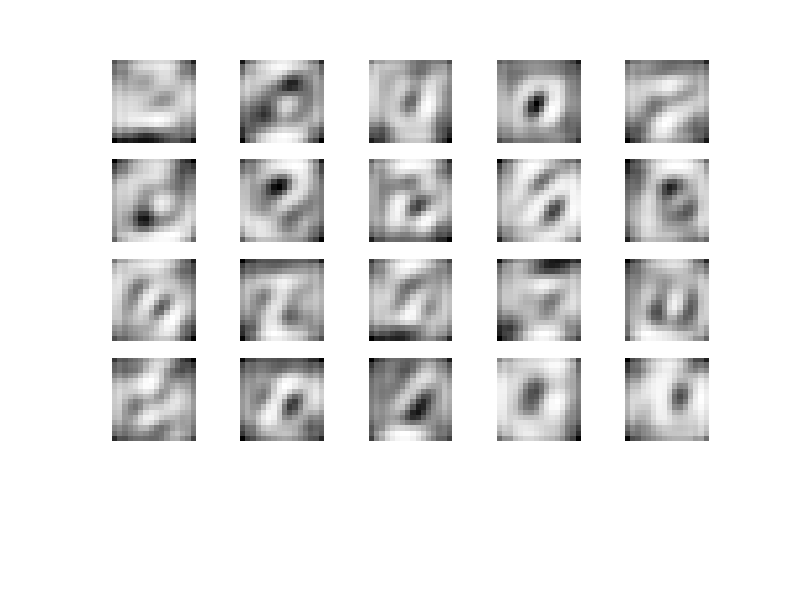
\includegraphics[width=0.7\textwidth]{imgs/weights_rbm.png} 
    \caption{Visuallized filters $16 \times 16$ filters of the first layer convolutional RBM of a DBN trained on MNIST.}
	\label{fig:rbmw}
\end{figure}

In the end the DBN reaches a classification performance of $82.45$ \%. 
This could be further improved by increasing the training time, fine-tuning the structure and parameters of the training algorithm of the DBN, which was not the focus point of this thesis.
An intentionally simple DBN structure was chosen due to the computational effort necessary to simulate the DBN as a spiking neural network. 


\subsubsection{Conversion comparison}

For the comparison of the conversion methods, we convert the RBM to its spiking counter parts, as described in 5.2 . 
The input rate of the images are converted to Poisson spike-trains, with a maximal frequency of $\lambda = 100 \text{Hz}$ .
Each input sample is simulated for $500 \text{ms}$, but we'll inspect how the simulated timespan effects the output.
Since the simulation time of one sample can take more the 1 minute, we evaluate all approaches on the same randomly drawn subset of the test set consisting of $100$ samples.

A visual inspection of the activations can be seen in Fig x. 
It is quite apparent, that all approaches capture the basic activation characteristics. 
While the conversion as a DBN is able to simulate the activation probabilities more closely to the original DBN, the spiking CNN show similar performance by a more deterministic behaviour replicating only the essential activation structure.
To quantify those differences we calculate the Kullback-Leibler divergence between the activation, as seen in Table x.

%TODO different sorting (layer wise)


\begin{figure}
	\centering
	\begin{subfigure}[t]{.32\textwidth}
  		\centering
  		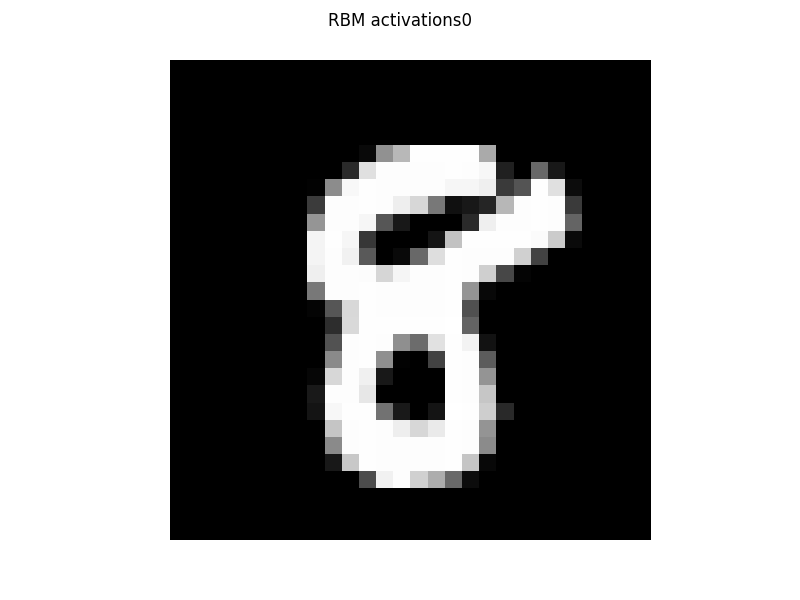
\includegraphics[width=.9\linewidth]{imgs/convert/rbm00000.png}
  		\caption{Input data.}
  		\label{fig:sub1}
	\end{subfigure}%
	\begin{subfigure}[t]{.32\textwidth}
  		\centering
  		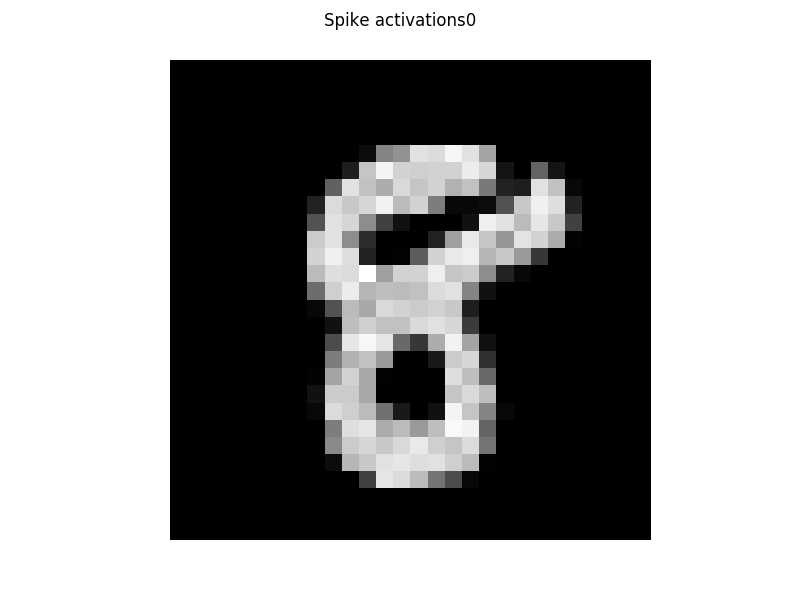
\includegraphics[width=.9\linewidth]{imgs/convert/cnn00000.png}
  		\caption{Spike input.}
  		\label{fig:sub2}
	\end{subfigure}
	
	\begin{subfigure}[t]{.24\textwidth}
  		\centering
  		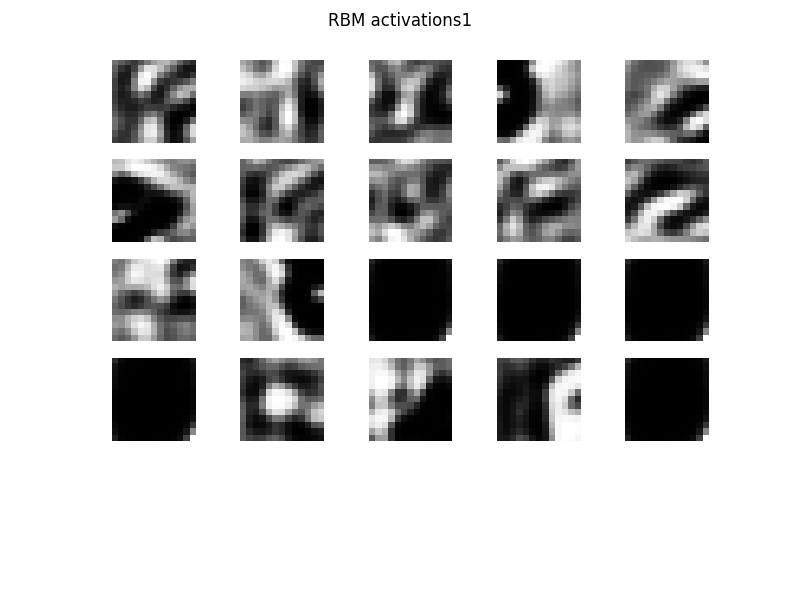
\includegraphics[width=.9\linewidth]{imgs/convert/rbm00001.png}
  		\label{fig:sub1}
	\end{subfigure}%
	\begin{subfigure}[t]{.24\textwidth}
  		\centering
  		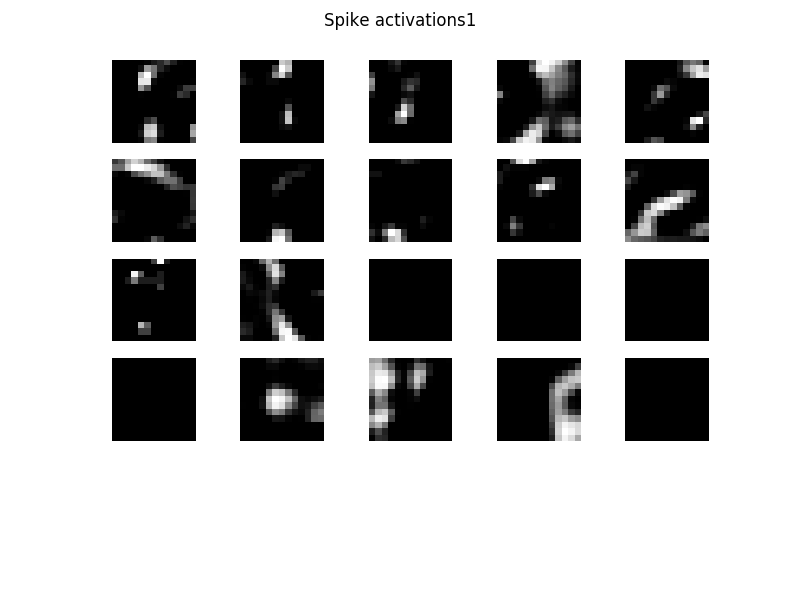
\includegraphics[width=.9\linewidth]{imgs/convert/cnn00001.png}
  		\label{fig:sub2}
	\end{subfigure}
	\begin{subfigure}[t]{.24\textwidth}
  		\centering
  		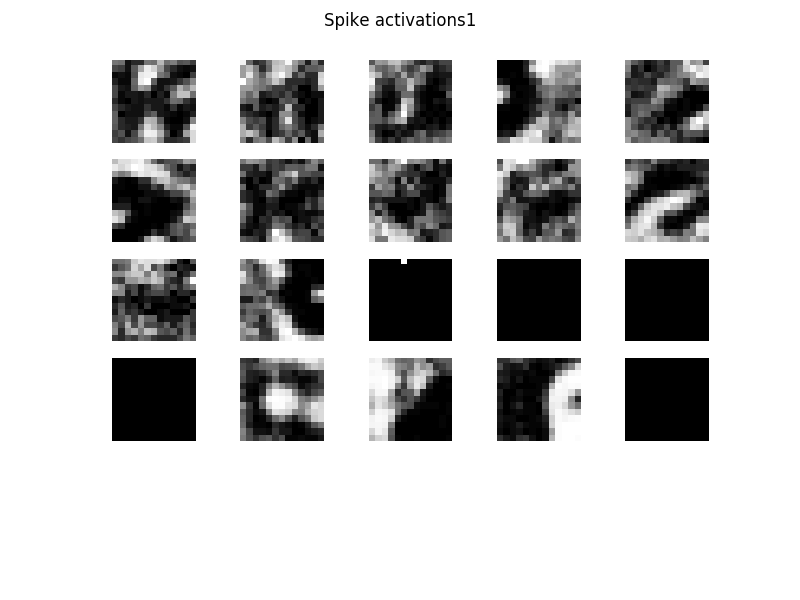
\includegraphics[width=.9\linewidth]{imgs/convert/coba00001.png}
  		\label{fig:sub2}
	\end{subfigure}
	\begin{subfigure}[t]{.24\textwidth}
  		\centering
  		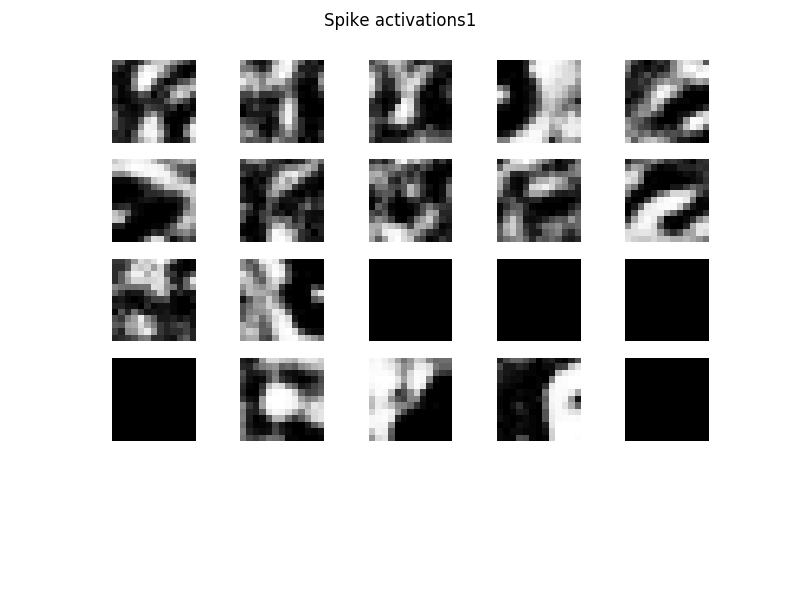
\includegraphics[width=.9\linewidth]{imgs/convert/cuba00001.png}
  		\label{fig:sub2}
	\end{subfigure}	

	\begin{subfigure}[t]{.24\textwidth}
  		\centering
  		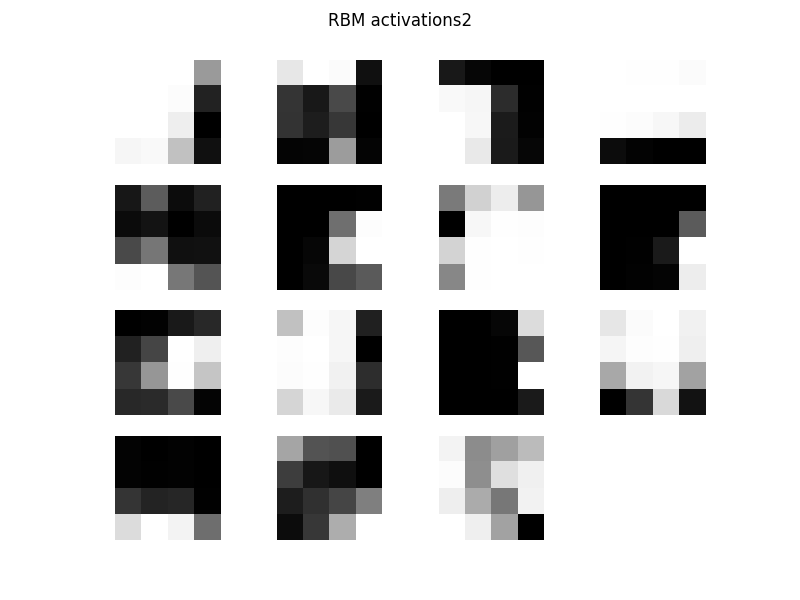
\includegraphics[width=.9\linewidth]{imgs/convert/rbm00002.png}
  		\label{fig:sub1}
	\end{subfigure}%
	\begin{subfigure}[t]{.24\textwidth}
  		\centering
  		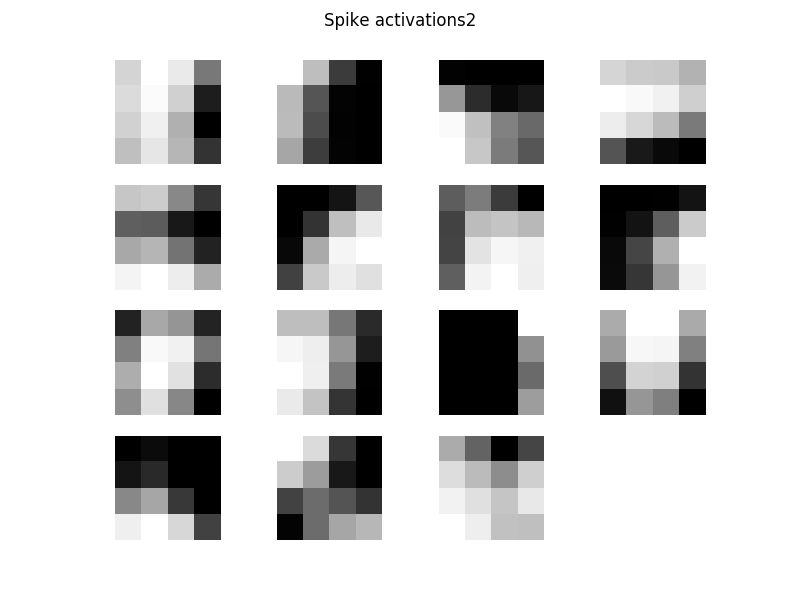
\includegraphics[width=.9\linewidth]{imgs/convert/cnn00002.png}
  		\label{fig:sub2}
	\end{subfigure}
	\begin{subfigure}[t]{.24\textwidth}
  		\centering
  		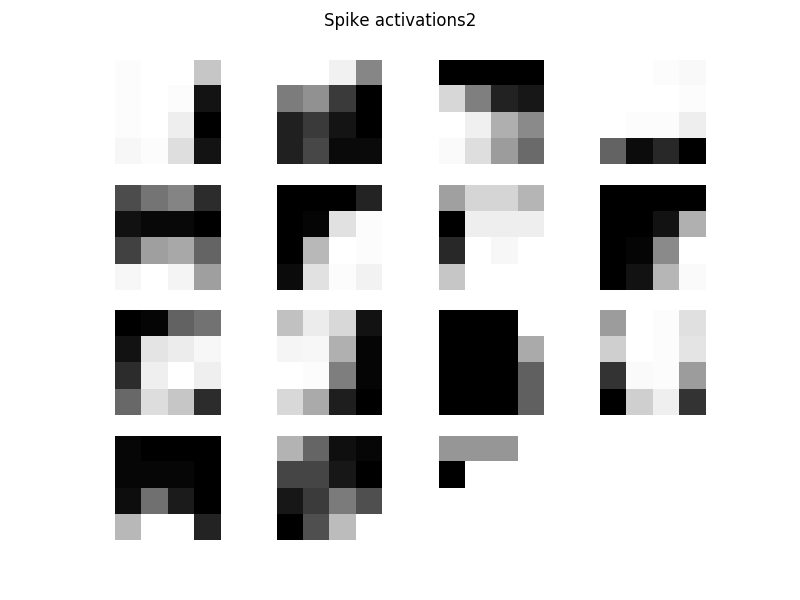
\includegraphics[width=.9\linewidth]{imgs/convert/coba00002.png}
  		\label{fig:sub2}
	\end{subfigure}
	\begin{subfigure}[t]{.24\textwidth}
  		\centering
  		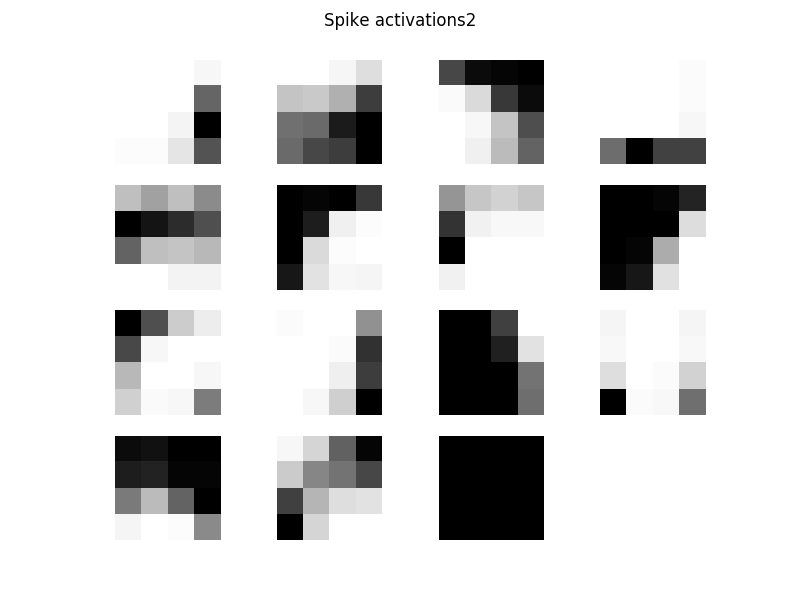
\includegraphics[width=.9\linewidth]{imgs/convert/cuba00002.png}
  		\label{fig:sub2}
	\end{subfigure}	

	\begin{subfigure}[t]{.24\textwidth}
  		\centering
  		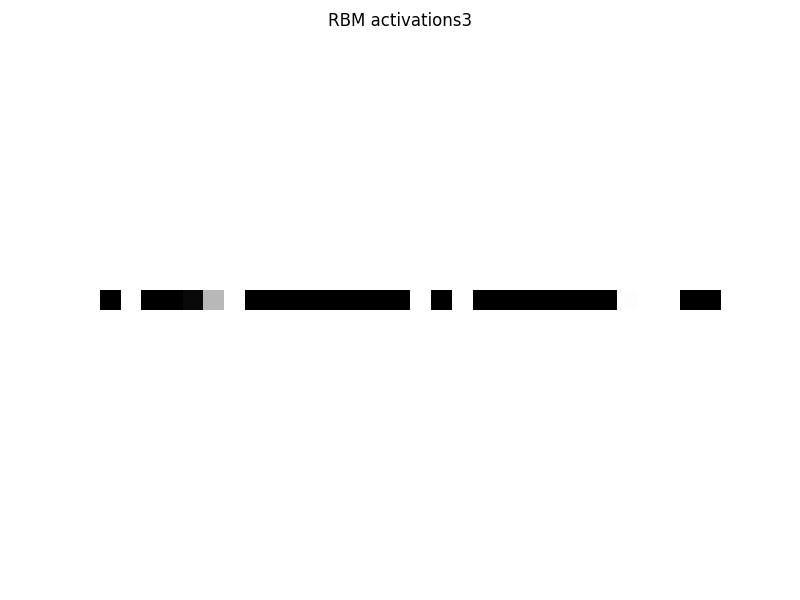
\includegraphics[width=.9\linewidth]{imgs/convert/rbm00003.png}
  		\label{fig:sub1}
	\end{subfigure}%
	\begin{subfigure}[t]{.24\textwidth}
  		\centering
  		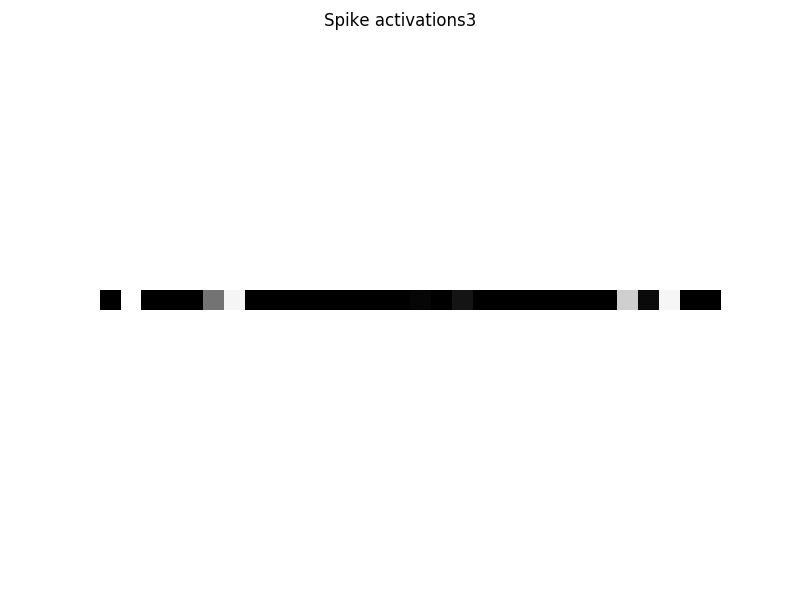
\includegraphics[width=.9\linewidth]{imgs/convert/cnn00003.png}
  		\label{fig:sub2}
	\end{subfigure}
	\begin{subfigure}[t]{.24\textwidth}
  		\centering
  		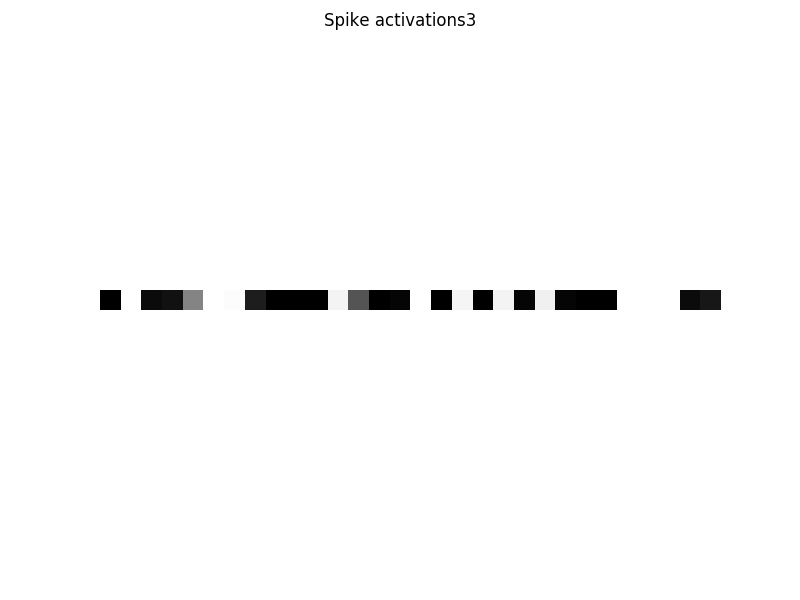
\includegraphics[width=.9\linewidth]{imgs/convert/coba00003.png}
  		\label{fig:sub2}
	\end{subfigure}
	\begin{subfigure}[t]{.24\textwidth}
  		\centering
  		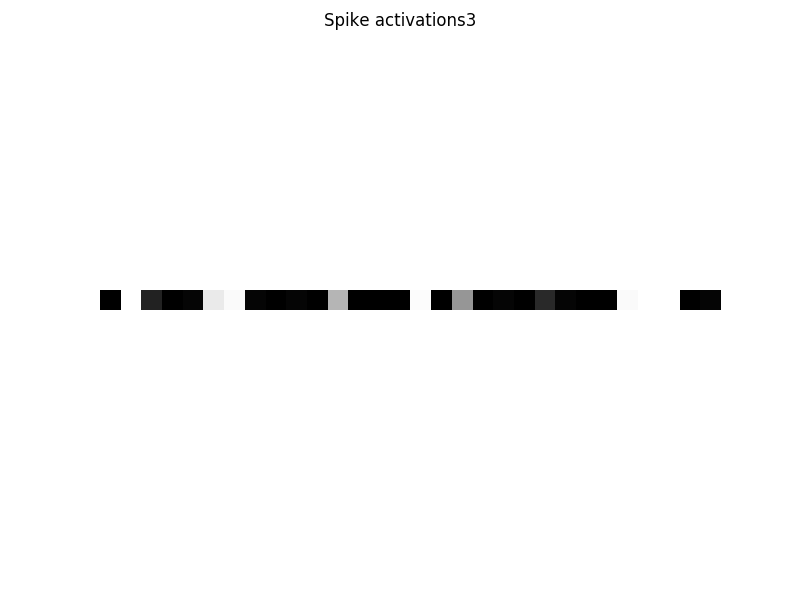
\includegraphics[width=.9\linewidth]{imgs/convert/cuba00003.png}
  		\label{fig:sub2}
	\end{subfigure}	
	
	\begin{subfigure}[t]{.24\textwidth}
  		\centering
  		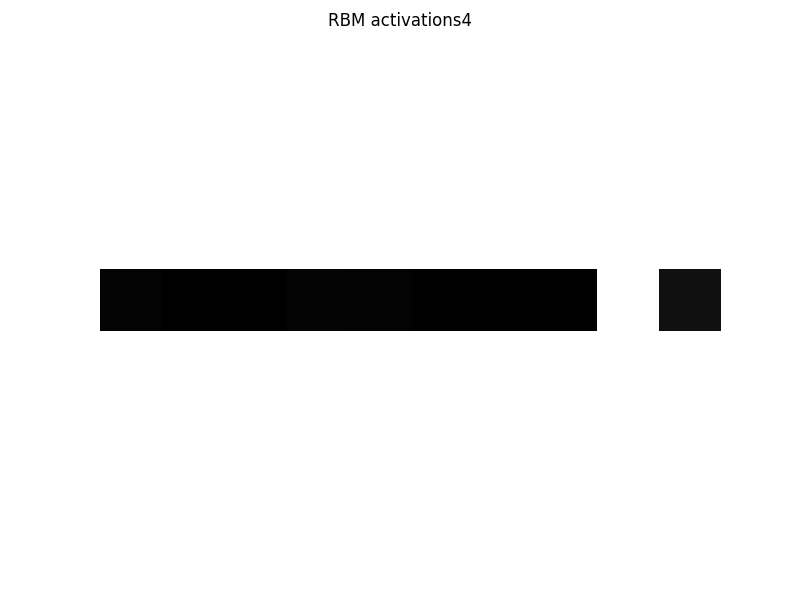
\includegraphics[width=.9\linewidth]{imgs/convert/rbm00004.png}
  		\caption{RBM.}
  		\label{fig:sub1}
	\end{subfigure}%
	\begin{subfigure}[t]{.24\textwidth}
  		\centering
  		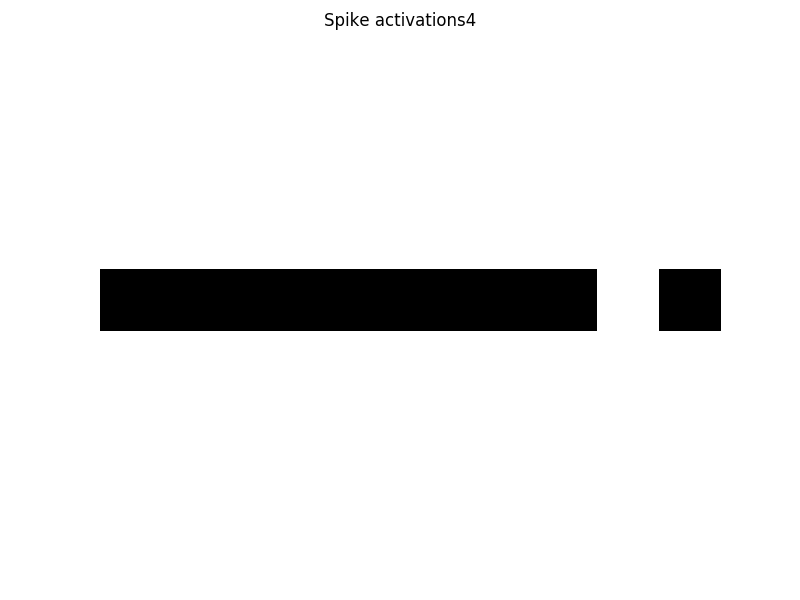
\includegraphics[width=.9\linewidth]{imgs/convert/cnn00004.png}
  		\caption{CNN.}
  		\label{fig:sub2}
	\end{subfigure}
	\begin{subfigure}[t]{.24\textwidth}
  		\centering
  		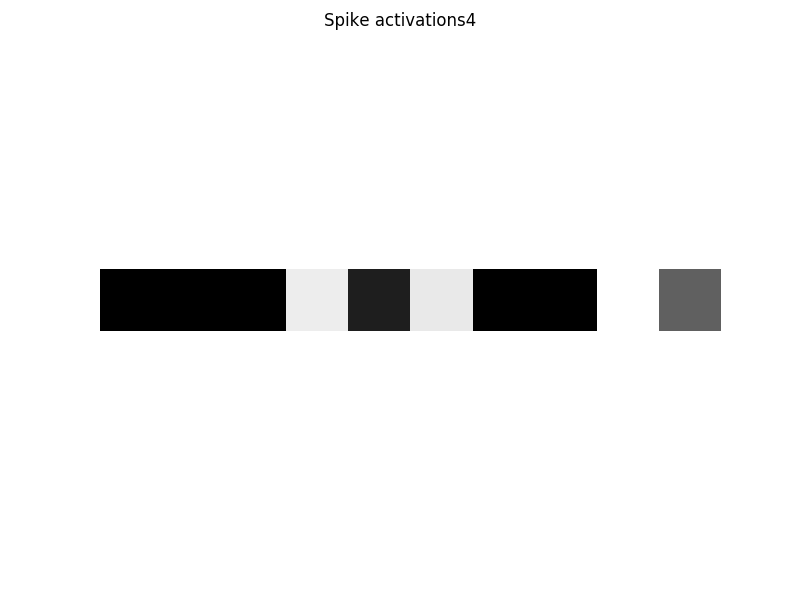
\includegraphics[width=.9\linewidth]{imgs/convert/coba00004.png}
  		\caption{COBA LIF DBN.}
  		\label{fig:sub2}
	\end{subfigure}
	\begin{subfigure}[t]{.24\textwidth}
  		\centering
  		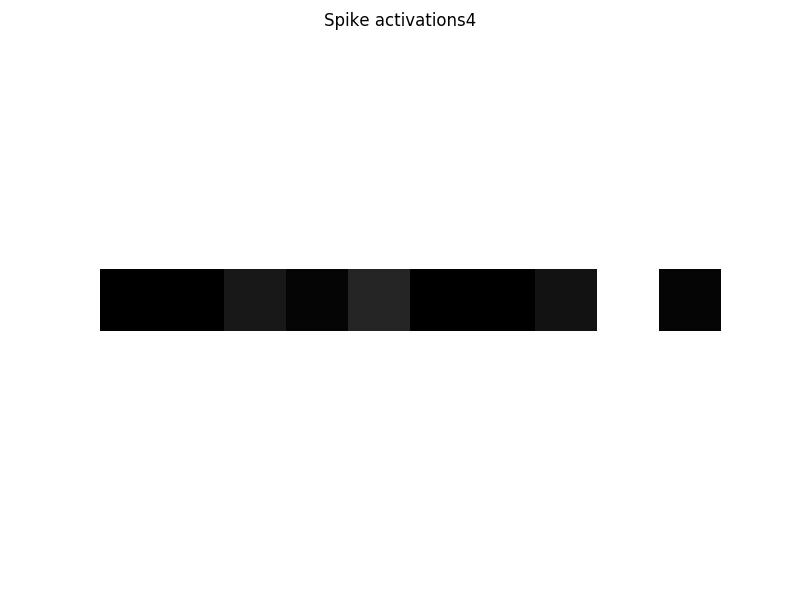
\includegraphics[width=.9\linewidth]{imgs/convert/cuba00004.png}
  		\caption{CUBA LIF DBN.}
  		\label{fig:sub2}
	\end{subfigure}	
	\caption{Activations in the features maps in a classical convolutional RBM. }
	\label{fig:stripes}
\end{figure}
%
%\begin{figure}
%	\centering
%	\begin{subfigure}[t]{.32\textwidth}
%  		\centering
%  		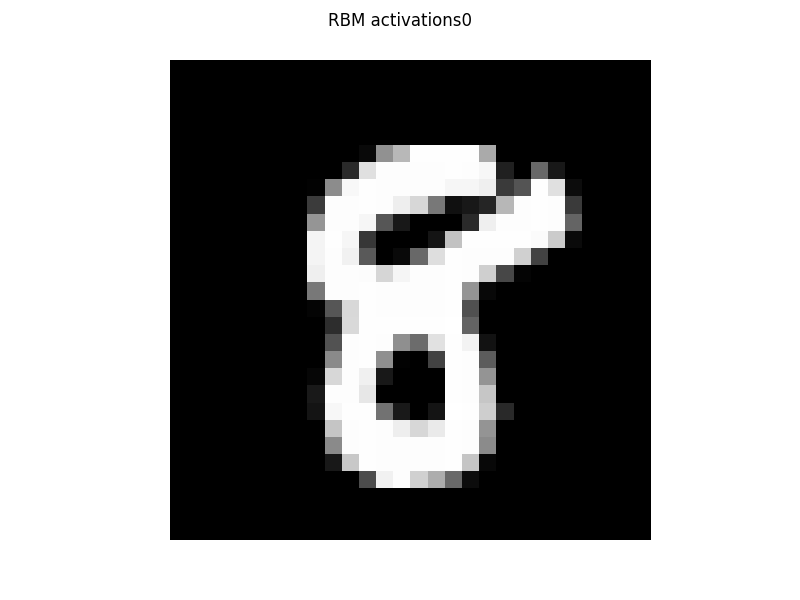
\includegraphics[width=.9\linewidth]{imgs/convert/rbm00000.png}
%  		\caption{Input data.}
%  		\label{fig:sub1}
%	\end{subfigure}%
%	\begin{subfigure}[t]{.32\textwidth}
%  		\centering
%  		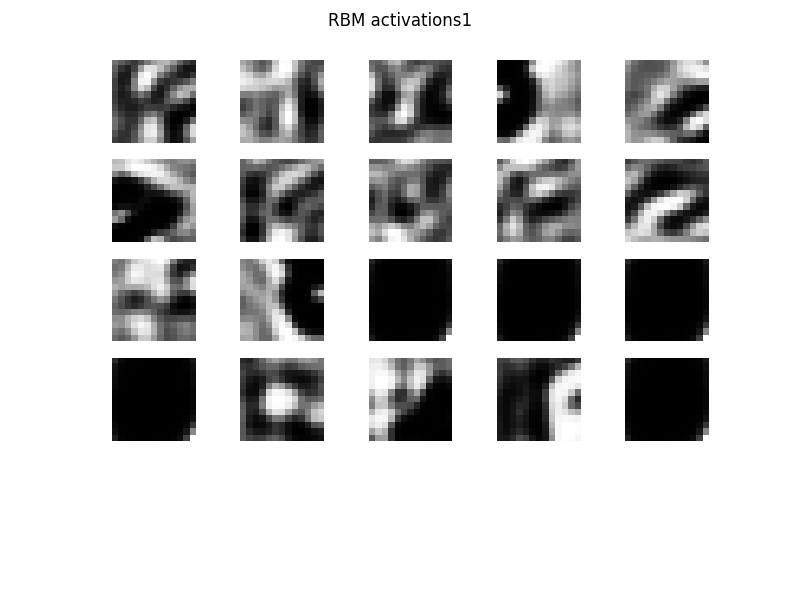
\includegraphics[width=.9\linewidth]{imgs/convert/rbm00001.png}
%  		\caption{Activations in the features maps of the first RBM layer.}
%  		\label{fig:sub2}
%	\end{subfigure}
%	\begin{subfigure}[t]{.32\textwidth}
%  		\centering
%  		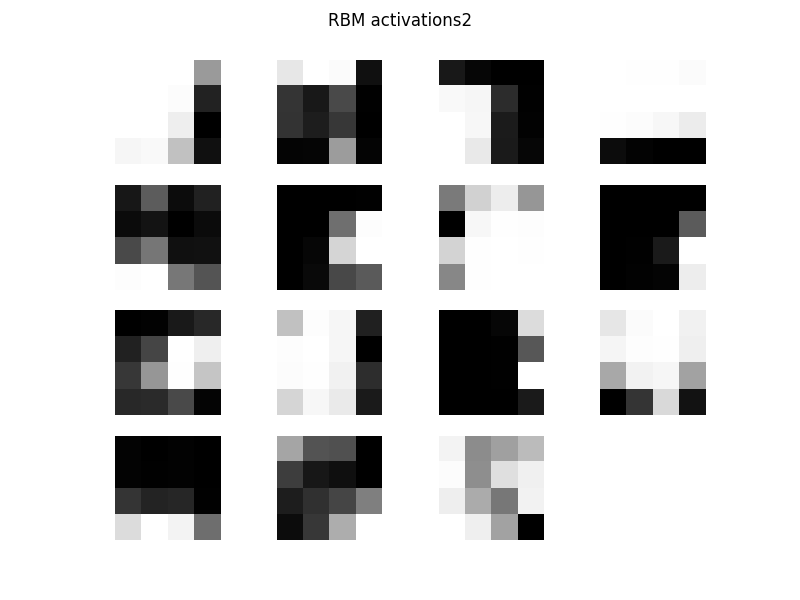
\includegraphics[width=.9\linewidth]{imgs/convert/rbm00002.png}
%  		\caption{Activations in the features maps of the second RBM layer.}
%  		\label{fig:sub2}
%	\end{subfigure}
%	\begin{subfigure}[t]{.32\textwidth}
%  		\centering
%  		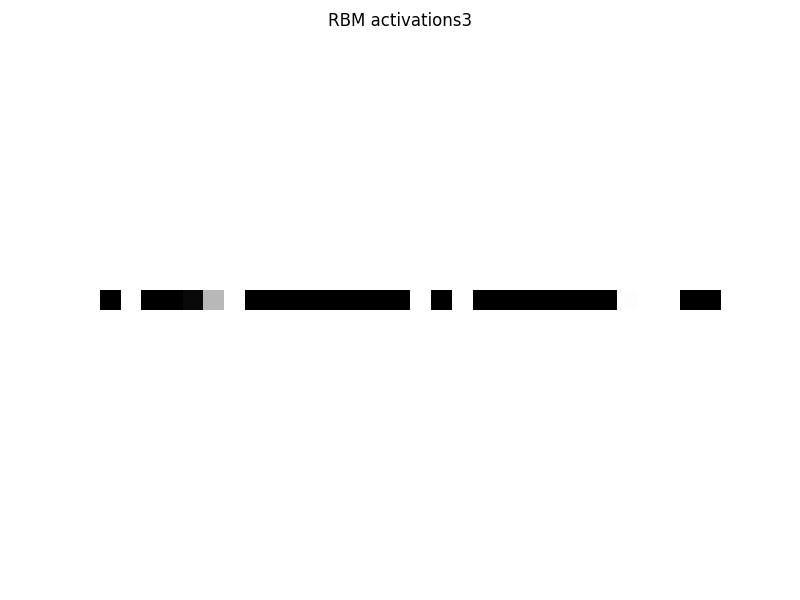
\includegraphics[width=.9\linewidth]{imgs/convert/rbm00003.png}
%  		\caption{Activations in the features maps of the third RBM layer.}
%  		\label{fig:sub2}
%	\end{subfigure}	
%	\begin{subfigure}[t]{.32\textwidth}
%  		\centering
%  		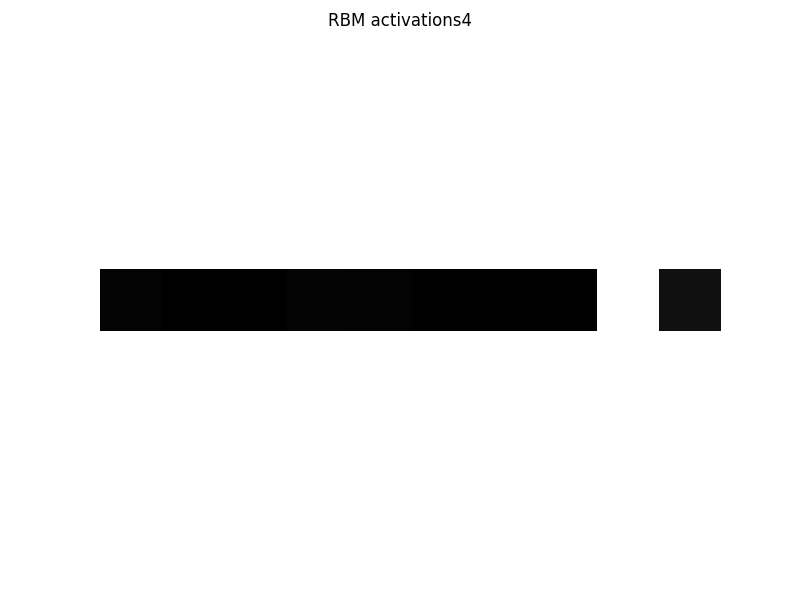
\includegraphics[width=.9\linewidth]{imgs/convert/rbm00004.png}
%  		\caption{Activations in the features maps of the fourth/label layer.}
%  		\label{fig:sub2}
%	\end{subfigure}
%	\caption{Activations in the features maps in a classical convolutional RBM. }
%	\label{fig:stripes}
%\end{figure}
%
%\begin{figure}
%	\centering
%	\begin{subfigure}[t]{.32\textwidth}
%  		\centering
%  		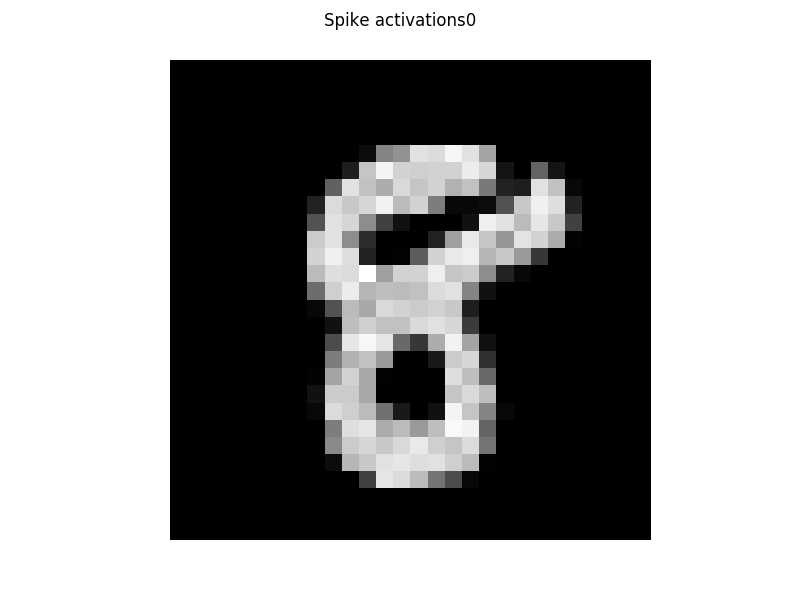
\includegraphics[width=.9\linewidth]{imgs/convert/cnn00000.png}
%  		\caption{Input data.}
%  		\label{fig:sub1}
%	\end{subfigure}%
%	\begin{subfigure}[t]{.32\textwidth}
%  		\centering
%  		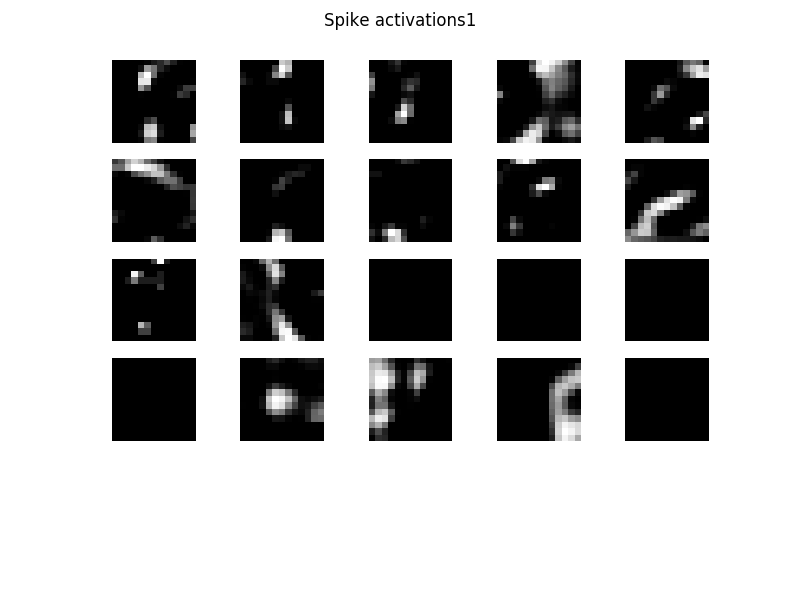
\includegraphics[width=.9\linewidth]{imgs/convert/cnn00001.png}
%  		\caption{Activations in the features maps of the first RBM layer.}
%  		\label{fig:sub2}
%	\end{subfigure}
%	\begin{subfigure}[t]{.32\textwidth}
%  		\centering
%  		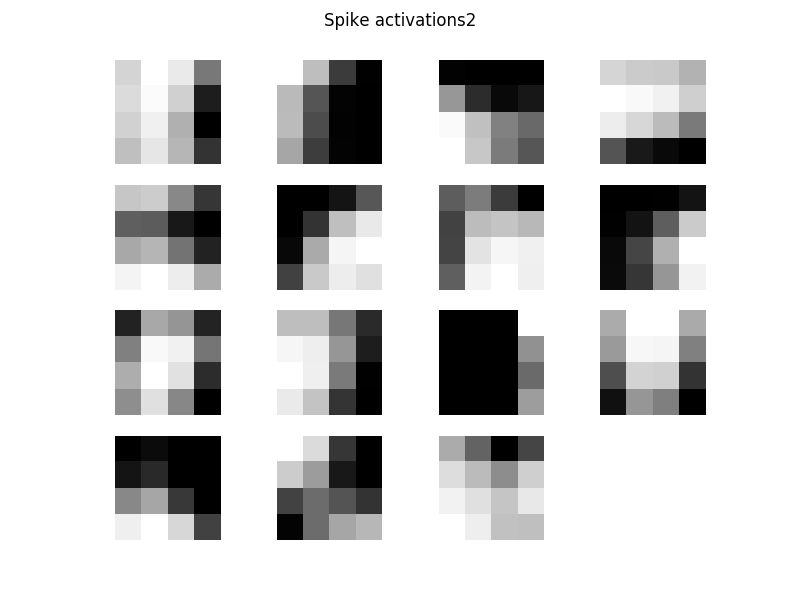
\includegraphics[width=.9\linewidth]{imgs/convert/cnn00002.png}
%  		\caption{Activations in the features maps of the second RBM layer.}
%  		\label{fig:sub2}
%	\end{subfigure}
%	\begin{subfigure}[t]{.32\textwidth}
%  		\centering
%  		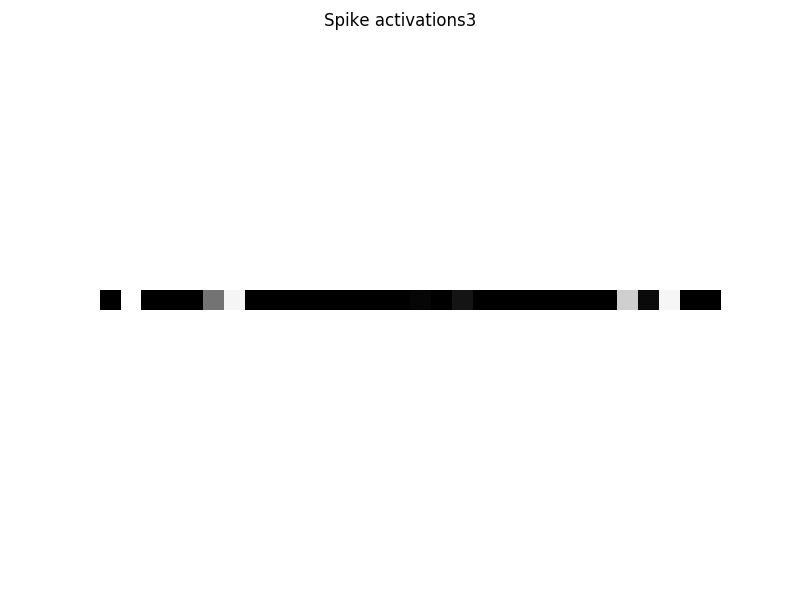
\includegraphics[width=.9\linewidth]{imgs/convert/cnn00003.png}
%  		\caption{Activations in the features maps of the third RBM layer.}
%  		\label{fig:sub2}
%	\end{subfigure}	
%	\begin{subfigure}[t]{.32\textwidth}
%  		\centering
%  		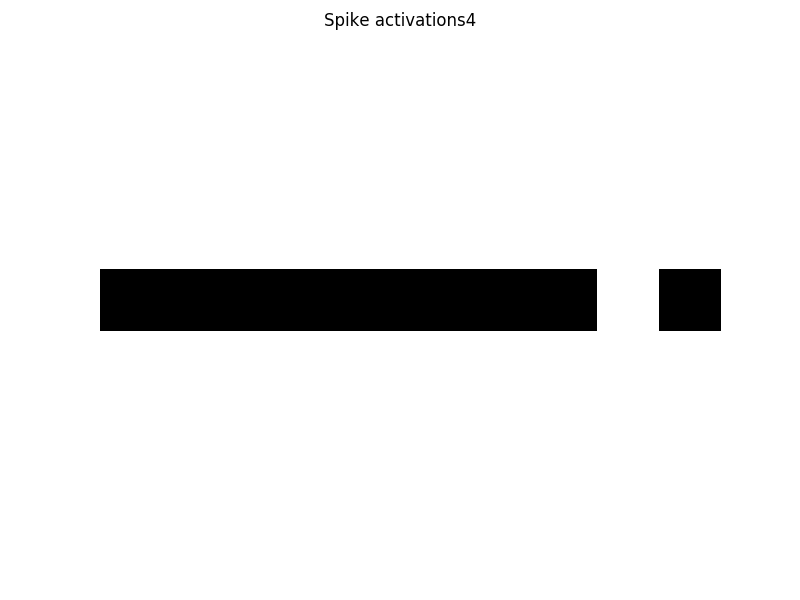
\includegraphics[width=.9\linewidth]{imgs/convert/cnn00004.png}
%  		\caption{Activations in the features maps of the fourth/label layer.}
%  		\label{fig:sub2}
%	\end{subfigure}
%	\caption{Activations in the features maps in the as CNN converted RBM. }
%	\label{fig:stripes}
%\end{figure}
%
%\begin{figure}
%	\centering
%	\begin{subfigure}[t]{.32\textwidth}
%  		\centering
%  		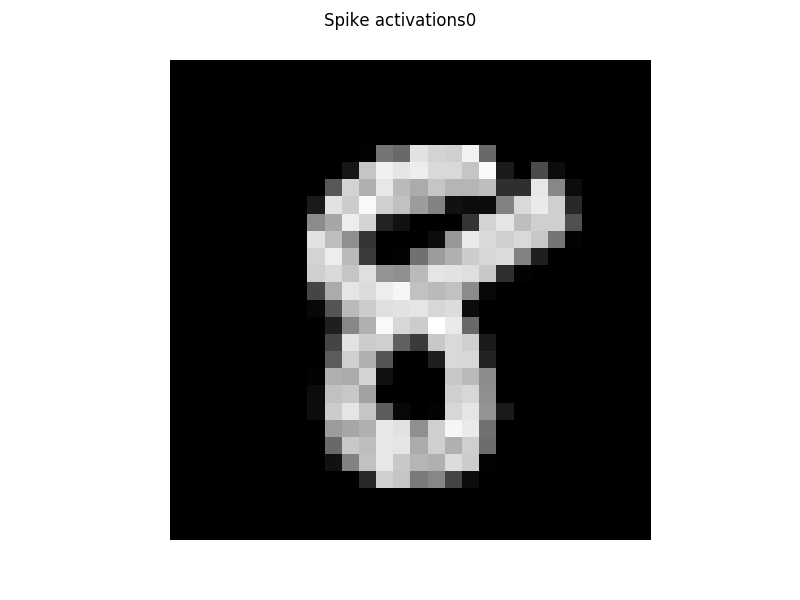
\includegraphics[width=.9\linewidth]{imgs/convert/coba00000.png}
%  		\caption{Input data.}
%  		\label{fig:sub1}
%	\end{subfigure}%
%	\begin{subfigure}[t]{.32\textwidth}
%  		\centering
%  		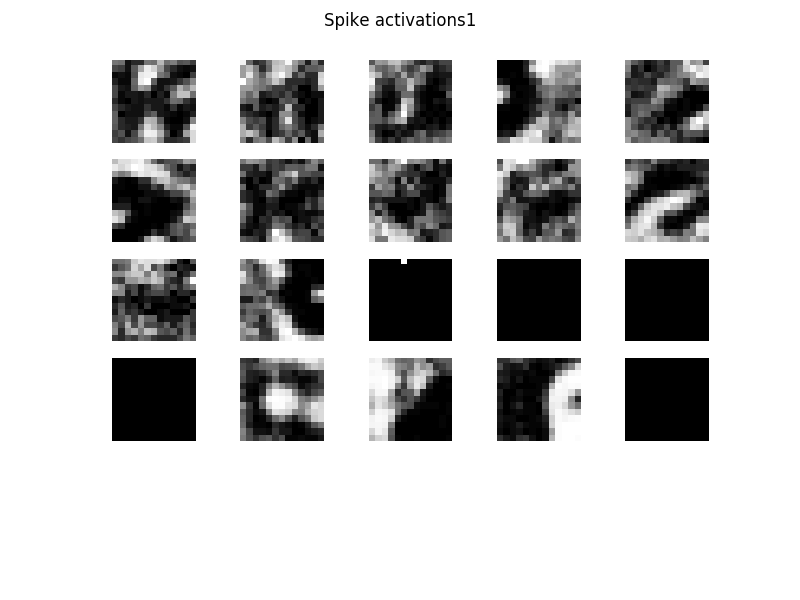
\includegraphics[width=.9\linewidth]{imgs/convert/coba00001.png}
%  		\caption{Activations in the features maps of the first RBM layer.}
%  		\label{fig:sub2}
%	\end{subfigure}
%	\begin{subfigure}[t]{.32\textwidth}
%  		\centering
%  		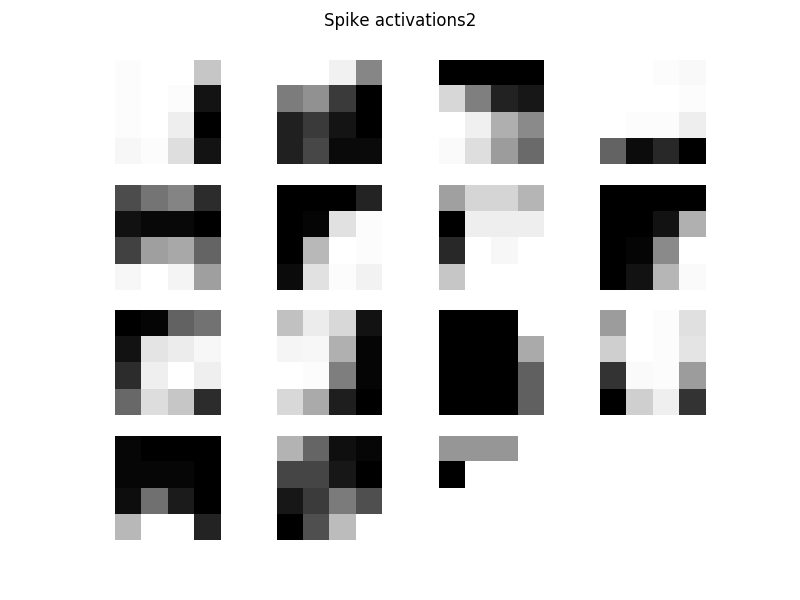
\includegraphics[width=.9\linewidth]{imgs/convert/coba00002.png}
%  		\caption{Activations in the features maps of the second RBM layer.}
%  		\label{fig:sub2}
%	\end{subfigure}
%	\begin{subfigure}[t]{.32\textwidth}
%  		\centering
%  		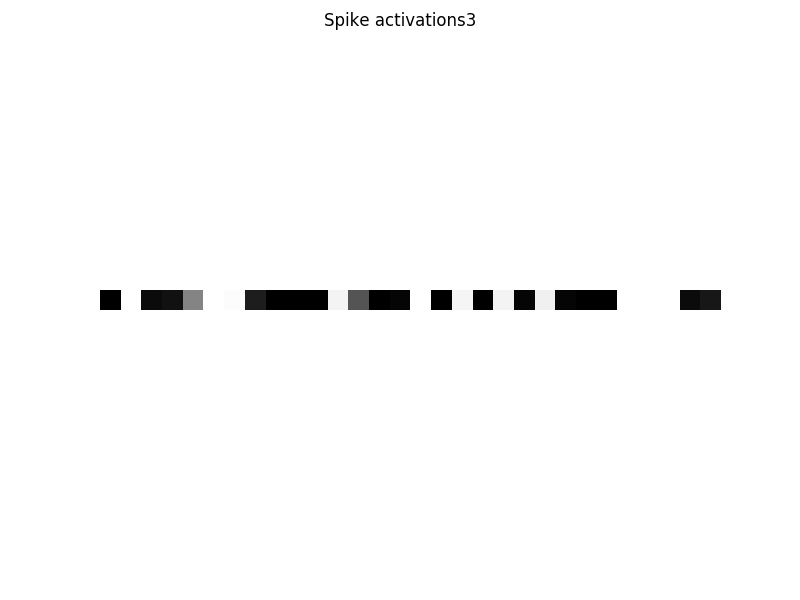
\includegraphics[width=.9\linewidth]{imgs/convert/coba00003.png}
%  		\caption{Activations in the features maps of the third RBM layer.}
%  		\label{fig:sub2}
%	\end{subfigure}	
%	\begin{subfigure}[t]{.32\textwidth}
%  		\centering
%  		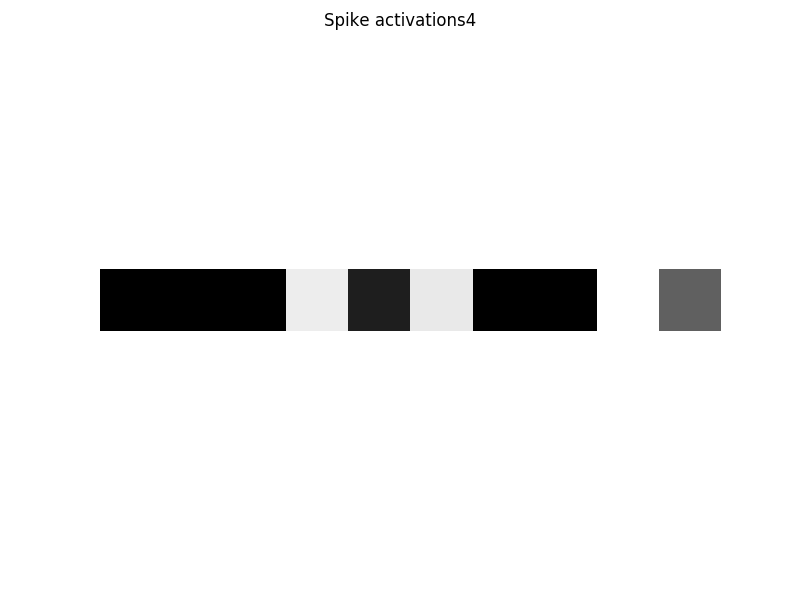
\includegraphics[width=.9\linewidth]{imgs/convert/coba00004.png}
%  		\caption{Activations in the features maps of the fourth/label layer.}
%  		\label{fig:sub2}
%	\end{subfigure}
%	\caption{Activations in the features maps in a as DBN converted RBM with conductance based LIF neurons. }
%	\label{fig:stripes}
%\end{figure}
%
%\begin{figure}
%	\centering
%	\begin{subfigure}[t]{.32\textwidth}
%  		\centering
%  		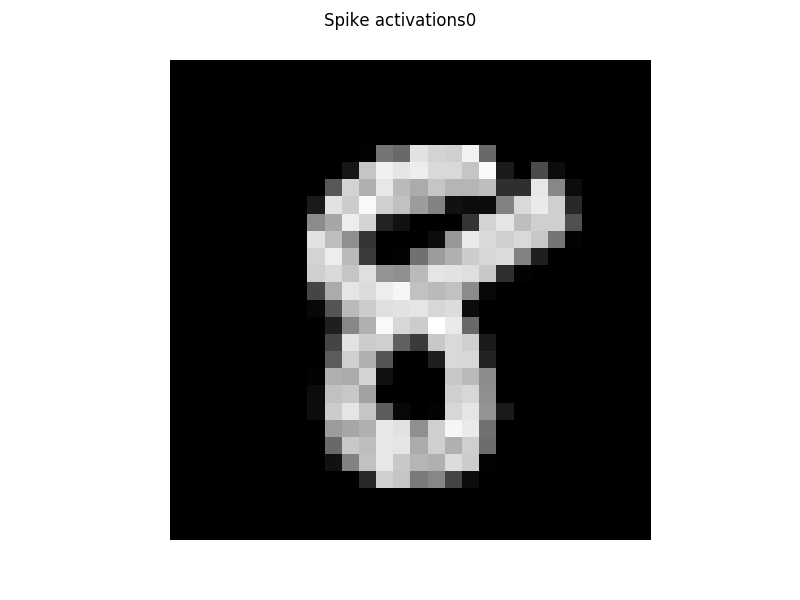
\includegraphics[width=.9\linewidth]{imgs/convert/cuba00000.png}
%  		\caption{Input data.}
%  		\label{fig:sub1}
%	\end{subfigure}%
%	\begin{subfigure}[t]{.32\textwidth}
%  		\centering
%  		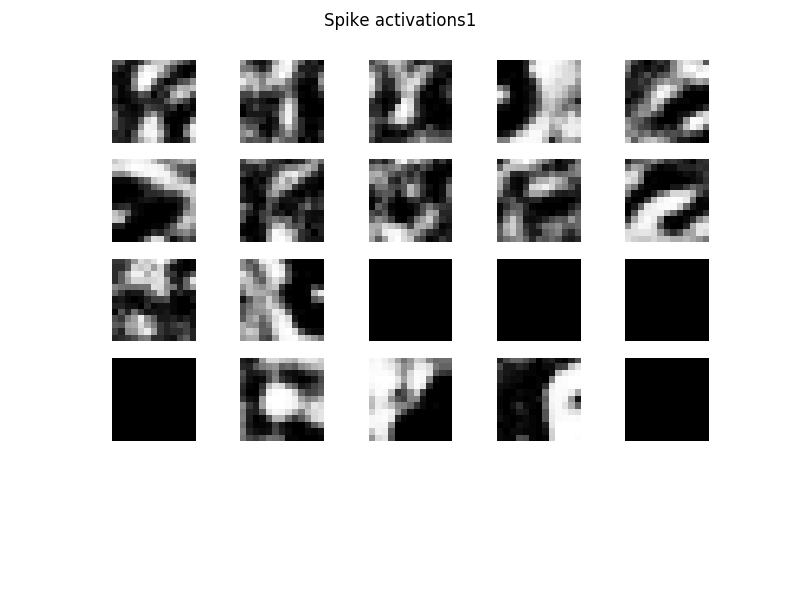
\includegraphics[width=.9\linewidth]{imgs/convert/cuba00001.png}
%  		\caption{Activations in the features maps of the first RBM layer.}
%  		\label{fig:sub2}
%	\end{subfigure}
%	\begin{subfigure}[t]{.32\textwidth}
%  		\centering
%  		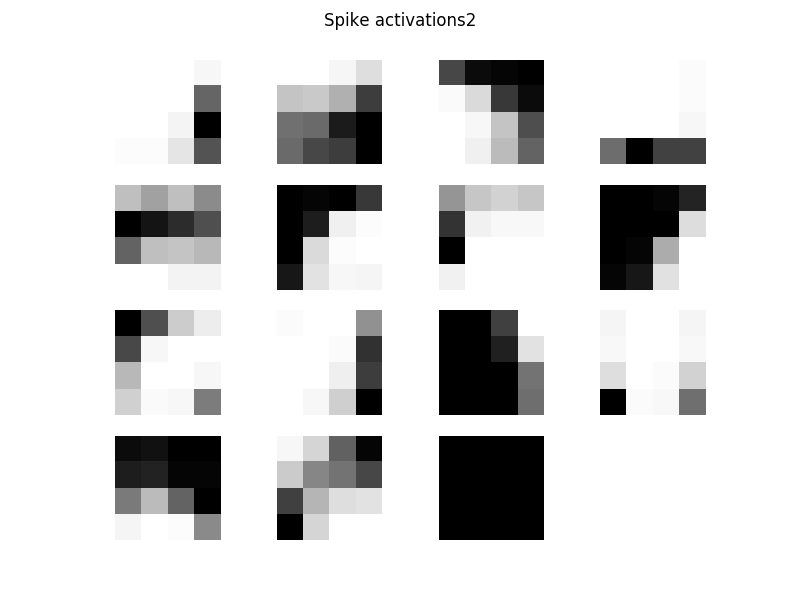
\includegraphics[width=.9\linewidth]{imgs/convert/cuba00002.png}
%  		\caption{Activations in the features maps of the second RBM layer.}
%  		\label{fig:sub2}
%	\end{subfigure}
%	\begin{subfigure}[t]{.32\textwidth}
%  		\centering
%  		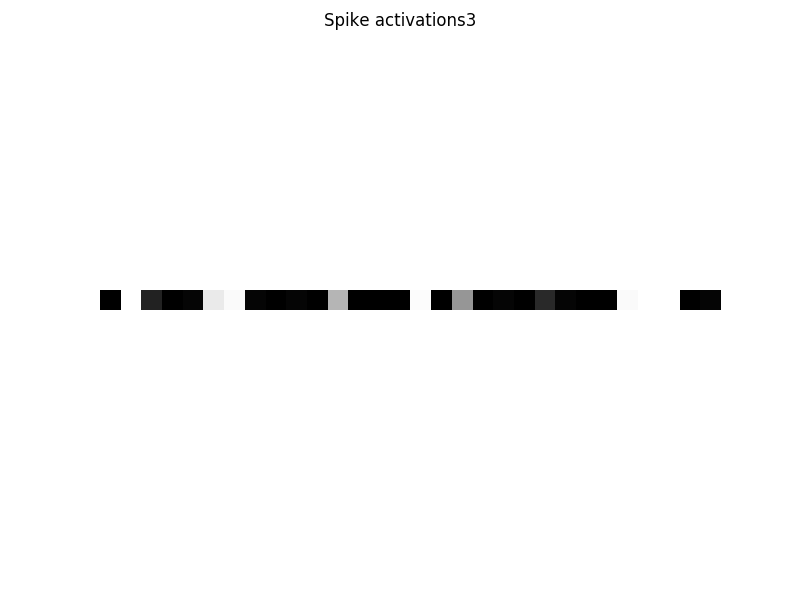
\includegraphics[width=.9\linewidth]{imgs/convert/cuba00003.png}
%  		\caption{Activations in the features maps of the third RBM layer.}
%  		\label{fig:sub2}
%	\end{subfigure}	
%	\begin{subfigure}[t]{.32\textwidth}
%  		\centering
%  		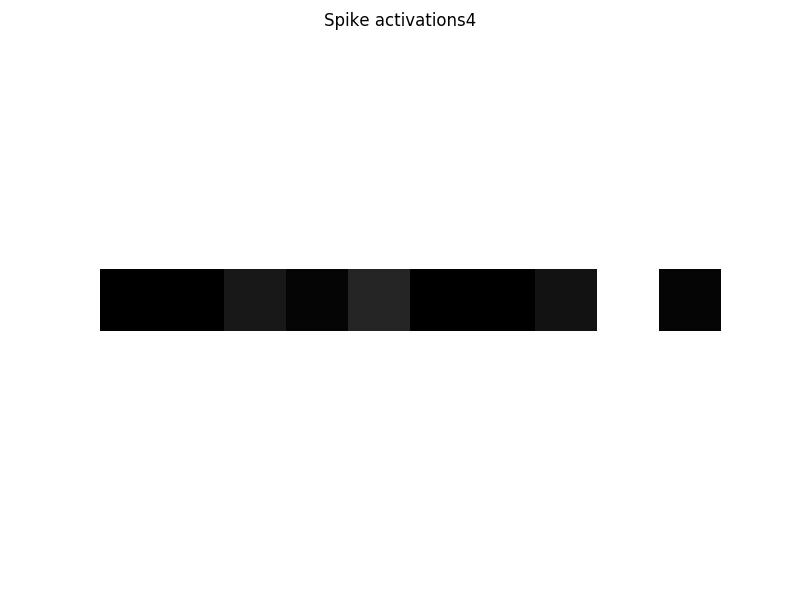
\includegraphics[width=.9\linewidth]{imgs/convert/cuba00004.png}
%  		\caption{Activations in the features maps of the fourth/label layer.}
%  		\label{fig:sub2}
%	\end{subfigure}
%	\caption{Activations in the features maps in a as DBN converted RBM with current based LIF neurons. }
%	\label{fig:stripes}
%\end{figure}

The performance on the sub dataset can be seen in Table x.
It is apparent, that all show similar performance. Interestingly the spiking DBN sometimes shows better performance than the RBM.
Most misclassifications can be from a human perspective been categorized as "reasonable" mistakes (as seen in Fig x) and hint, that further fine-tuning the DBN could resolve some misclassifications.

Another factor is the simulated runtime for each sample. It is quite apparent from table x (Table: CNN vs CUBA , simulated time , performance, run time  ) that a longer classifcation time benefits the performance. But due to it's more deterministic nature the CNN approach shows less variations as the simulation time changes. 

\subsection{eCD}

To get an intuitive insight into the eCD algorithm, we'll visualize the positive and negative phase for the stripe dataset.
It is apparent, that in the positive phase a sample from the data distribution is learned and in the negative phase the model distribution is unlearned.
As the training progresses and the model distribution approximates the data distribution more closely the weight updates become smaller (figure). 

\begin{figure}[h!]
	\centering
	\begin{subfigure}[t]{.19\textwidth}
  		\centering
  		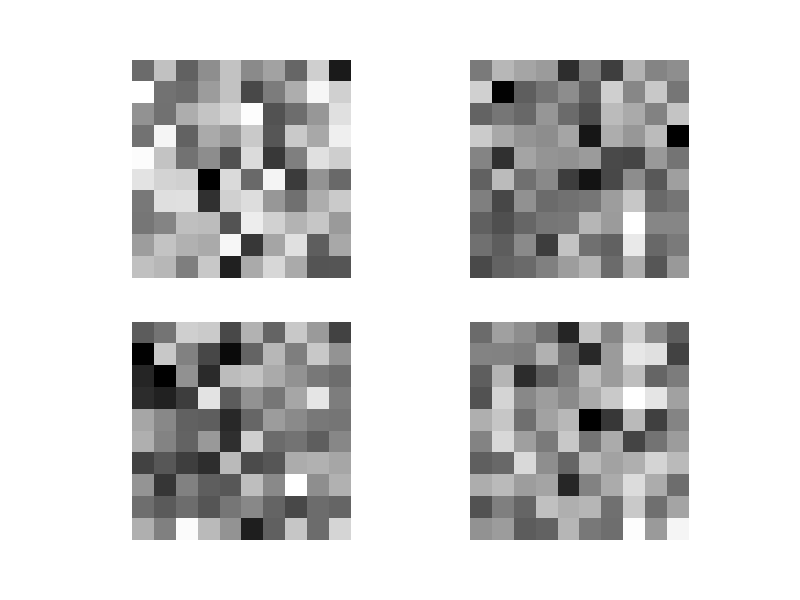
\includegraphics[width=\linewidth]{imgs/inspect/00010.png}
  		\label{fig:sub1}
	\end{subfigure}%
	\begin{subfigure}[t]{.19\textwidth}
  		\centering
  		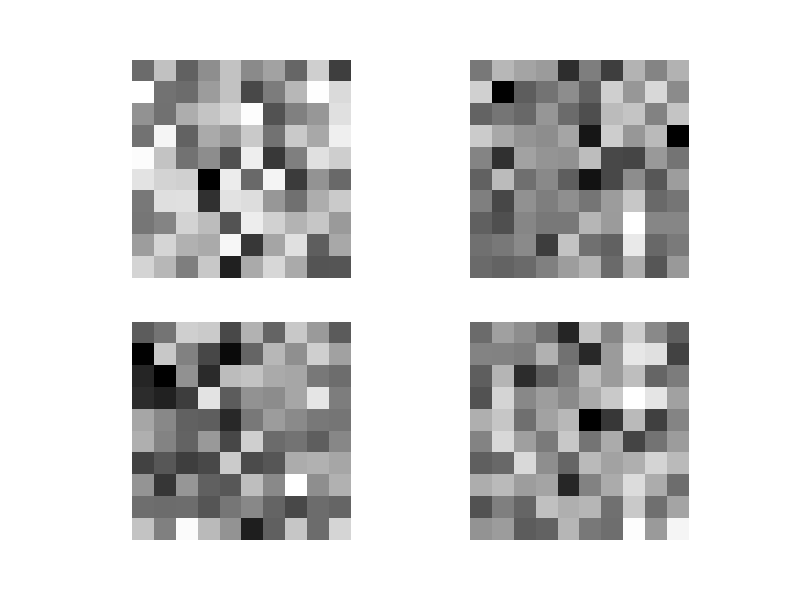
\includegraphics[width=\linewidth]{imgs/inspect/00011.png}
  		\label{fig:sub1}
	\end{subfigure}%
	\begin{subfigure}[t]{.19\textwidth}
  		\centering
  		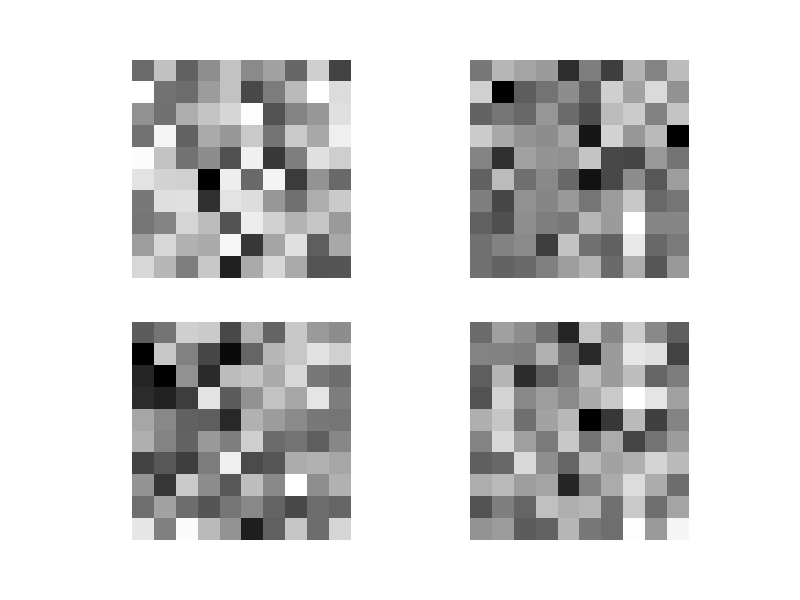
\includegraphics[width=\linewidth]{imgs/inspect/00012.png}
  		\label{fig:sub1}
	\end{subfigure}%
	\begin{subfigure}[t]{.19\textwidth}
  		\centering
  		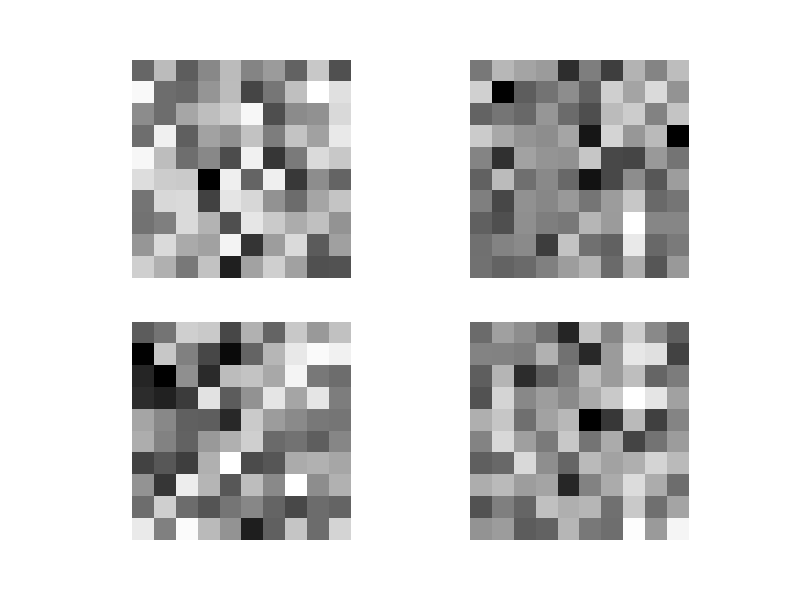
\includegraphics[width=\linewidth]{imgs/inspect/00013.png}
  		\label{fig:sub1}
	\end{subfigure}%
	\begin{subfigure}[t]{.19\textwidth}
  		\centering
  		\includegraphics[width=\linewidth]{imgs/inspect/00014.png}
  		\label{fig:sub1}
	\end{subfigure}%
	
	\begin{subfigure}[t]{.19\textwidth}
  		\centering
  		\includegraphics[width=\linewidth]{imgs/inspect/00015.png}
  		\label{fig:sub1}
	\end{subfigure}%
	\begin{subfigure}[t]{.19\textwidth}
  		\centering
  		\includegraphics[width=\linewidth]{imgs/inspect/00016.png}
  		\label{fig:sub1}
	\end{subfigure}%
	\begin{subfigure}[t]{.19\textwidth}
  		\centering
  		\includegraphics[width=\linewidth]{imgs/inspect/00017.png}
  		\label{fig:sub1}
	\end{subfigure}%
	\begin{subfigure}[t]{.19\textwidth}
  		\centering
  		\includegraphics[width=\linewidth]{imgs/inspect/00018.png}
  		\label{fig:sub1}
	\end{subfigure}%
	\caption{Positive phase and negative phase of a diagonal stripe with 4 filters. In the first 4 images the stripe is learned, while during the last 4 images the model distribution is unlearned.}
	\label{fig:stripes}
\end{figure}


\subsubsection{Hidden sparsity/ learning the data distribution}

To evaluate how good the model distribution matches the data distribution, we compare the input sample to the reconstruction obtained after the removing the input and letting the system settle towards it's model distribution.
In the beginning of the training the model distribution and thus the reconstruction is approximately random.
As the training progresses, the reconstruction matches the original input image more closely and thus the model distribution shifts towards the data distribution.

\begin{figure}[h!]
	\centering
	\begin{subfigure}{.25\textwidth}
  		\centering
  		\includegraphics[width=\linewidth]{imgs/reconst/00001.png}
  		\label{fig:sub1}
	\end{subfigure}%
	\begin{subfigure}{.25\textwidth}
  		\centering
  		\includegraphics[width=\linewidth]{imgs/reconst/00003.png}
  		\label{fig:sub1}
	\end{subfigure}%
	\begin{subfigure}{.25\textwidth}
  		\centering
  		\includegraphics[width=\linewidth]{imgs/reconst/00005.png}
  		\label{fig:sub1}
	\end{subfigure}%
	\begin{subfigure}{.25\textwidth}
  		\centering
  		\includegraphics[width=\linewidth]{imgs/reconst/00007.png}
  		\label{fig:sub1}
	\end{subfigure}%
	
	
	\begin{subfigure}{.25\textwidth}
  		\centering
  		\includegraphics[width=\linewidth]{imgs/reconst/00002.png}
  		\label{fig:sub1}
	\end{subfigure}%
	\begin{subfigure}{.25\textwidth}
  		\centering
  		\includegraphics[width=\linewidth]{imgs/reconst/00004.png}
  		\label{fig:sub1}
	\end{subfigure}%
	\begin{subfigure}{.25\textwidth}
  		\centering
  		\includegraphics[width=\linewidth]{imgs/reconst/00006.png}
  		\label{fig:sub1}
	\end{subfigure}%
	\begin{subfigure}{.25\textwidth}
  		\centering
  		\includegraphics[width=\linewidth]{imgs/reconst/00008.png}
  		\label{fig:sub1}
	\end{subfigure}%
	\caption{Positive phase and negative phase of a diagonal stripe with 4 filters. In the first 4 images the stripe is learned, while during the last 4 images the model distribution is unlearned.}
	\label{fig:stripes}
\end{figure}

In Addition the weights/ filters become more specialized, thus resulting in a sparse activation of the hidden layer as visualized in Figure x (start, end, curve).  
\\\\\\\\
\begin{figure}[h!]
	\centering
	\begin{subfigure}[t]{.32\textwidth}
  		\centering
  		\includegraphics[width=.9\linewidth]{imgs/reconst/00030_h.png}
  		\caption{Activations at the beginning.}
  		\label{fig:sub1}
	\end{subfigure}%
	\begin{subfigure}[t]{.32\textwidth}
  		\centering
  		\includegraphics[width=.9\linewidth]{imgs/reconst/00975_h.png}
  		\caption{Activations after some training.}
  		\label{fig:sub2}
	\end{subfigure}
	\begin{subfigure}[t]{.32\textwidth}
  		\centering
  		\includegraphics[width=.9\linewidth]{imgs/reconst/hact.png}
  		\caption{Total number of activations per sample over time.}
  		\label{fig:sub2}
	\end{subfigure}
	\caption{Activations in the features maps in a as DBN converted RBM with current based LIF neurons. }
	\label{fig:stripes}
\end{figure}


\subsubsection{Lateral connections}

An important addition to the convolution spiking RBM, are the lateral inhibitory connections in the hidden layer. 
Each neuron in the hidden layer at position $i,j$ in feature map $k$ is connected to other neurons in all other feature maps $K \ k$ at the approximatly same position $i', j'$ with $ |i'-i| \le 2 , |j' - j| \le 2 $.   
This results in faster training and more discriminative features and better results.

\begin{figure}[h!]
	\centering
	\begin{subfigure}[t]{.45\textwidth}
  		\centering
  		\includegraphics[width=.9\linewidth]{imgs/inhib/02129.png}
  		\caption{Weights without lateral inhibitory connections.}
  		\label{fig:sub1}
	\end{subfigure}%
	\begin{subfigure}[t]{.45\textwidth}
  		\centering
  		\includegraphics[width=.9\linewidth]{imgs/inhib/03023.png}
  		\caption{Weights with lateral inhibitory connections.}
  		\label{fig:sub2}
	\end{subfigure}
	\caption{$5 \times 5$ convolution filter matrices with and without lateral inhibitory connections in the top RBM layer on the stripe dataset. Whereas the filters without lateral connections look more similar the filters with lateral connections are more different and discriminative.}
	\label{fig:stripes}
\end{figure}

\subsubsection{Convolution vs no Convolution}

To demonstrate the benefits of convolution even on a small dataset we train two DBNs with the same number of free parameters, one convolutional , one without any convolution.
The parameters for the first layer are chosen to be $20$ and for the second "association" layer $250$.

For the convolution DBN this results in a structure of $3$ $7x7$ convolutional filters in the first layer, and a fully connected RBM with $5$ hidden units in the second layer.
For the DBN without convolution, this results in two fully connected RBM's, where the first RBM has $2$ hidden units and the second RBM has $120$ hidden units.

Both DBNs are trained with 100 samples for the first layer and 500 samples with labels for the second layer, since it has more free parameters.

The resulting weights are visuallized in Fig. X

\begin{figure}[h!]
	\centering
	\begin{subfigure}[t]{.45\textwidth}
  		\centering
  		\includegraphics[width=.9\linewidth]{imgs/cvsnc/wc.png}
  		\caption{Weights of the DBN with convolutions.}
  		\label{fig:sub1}
	\end{subfigure}%
	\begin{subfigure}[t]{.45\textwidth}
  		\centering
  		\includegraphics[width=.9\linewidth]{imgs/cvsnc/wnc.png}
  		\caption{Weights of the DBN without convolutions.}
  		\label{fig:sub2}
	\end{subfigure}
	\caption{Weight of the first layers of the DBNs with and without convolutions.}
	\label{fig:stripes}
\end{figure}


This suggests, that the DBN with convolution is able to capture the structure of the data better with the same number of free parameters. 
This also shows in the final classification results.
While the DBN without convolutions reaches its top performance of $60 \%$ after 500 samples, the convolutional DBN reaches its top performance of $100 \%$ already after being presented with 300 samples.
 

\subsubsection{Simulation time}

We also evaluate how the simulation time for one time step changes as the network complexity increases.
A network on the $10 \times 10$ pixel stripe dataset is run for 1 learning step and the time is measured.
As we increase the number of hidden units, the runtime increases more or less linearly (see Fig X).

\begin{figure}
	\centering
    	\includegraphics[width=0.7\textwidth]{imgs/runtime-1.png} 
    \caption{The runtime of a learning step in dependence on the size of the Network.}
	\label{fig:rbmw}
\end{figure}


\subsubsection{Performance on the stripe dataset}

Due to the training time, we train the a DBN on the stripe dataset. 
The DBN consists of two layers, with the first layer consisting of a convolutional RBM with $20$ $7 \times 7$ filters and the second layer being fully connected with $20$ hidden units.
The first layer is trained with $1000$ samples without labels.
The weights of the first layer are then keep fixed and the second layer is trained over $500$ samples with their corresponding labels.

\begin{figure}[h!]
	\centering
    	\includegraphics[width=0.7\textwidth]{imgs/dbn_stripe.png} 
    \caption{Abstract architecture of the DBN for the stripe dataset.}
	\label{fig:rbmw}
\end{figure}


\begin{figure}[h!]
	\centering
	\begin{subfigure}[t]{.45\textwidth}
  		\centering
  		\includegraphics[width=.9\linewidth]{imgs/7x7/w1.png}
  		\caption{Weights a the beginning of training.}
  		\label{fig:sub1}
	\end{subfigure}%
	\begin{subfigure}[t]{.45\textwidth}
  		\centering
  		\includegraphics[width=.9\linewidth]{imgs/7x7/w2.png}
  		\caption{Weights after 250 samples.}
  		\label{fig:sub2}
	\end{subfigure}
	\begin{subfigure}[t]{.45\textwidth}
  		\centering
  		\includegraphics[width=.9\linewidth]{imgs/7x7/w3.png}
  		\caption{Weights after 500 samples.}
  		\label{fig:sub2}
	\end{subfigure}
	\begin{subfigure}[t]{.45\textwidth}
  		\centering
  		\includegraphics[width=.9\linewidth]{imgs/7x7/w4.png}
  		\caption{Weights after 750 samples.}
  		\label{fig:sub2}
	\end{subfigure}
	\begin{subfigure}[t]{.45\textwidth}
  		\centering
  		\includegraphics[width=.9\linewidth]{imgs/7x7/w5.png}
  		\caption{Weights after 1000 samples.}
  		\label{fig:sub2}
	\end{subfigure}
	\caption{$5 \times 5$ convolution filter matrices development during training with $1000$ samples.}
	\label{fig:stripes}
\end{figure}



\begin{figure}[h!]
	\centering
	\begin{subfigure}[t]{.45\textwidth}
  		\centering
  		\includegraphics[width=.9\linewidth]{imgs/7x7/00006_v.png}
  		\caption{Visible layer activations in the beginning.}
  		\label{fig:sub1}
	\end{subfigure}%
	\begin{subfigure}[t]{.45\textwidth}
  		\centering
  		\includegraphics[width=.9\linewidth]{imgs/7x7/01992_v.png}
  		\caption{Visible layer  activations after 1000 samples.}
  		\label{fig:sub2}
	\end{subfigure}
	
	\begin{subfigure}[t]{.45\textwidth}
  		\centering
  		\includegraphics[width=.9\linewidth]{imgs/7x7/00006_h.png}
  		\caption{Hidden layer activations in the beginning.}
  		\label{fig:sub2}
	\end{subfigure}
	\begin{subfigure}[t]{.45\textwidth}
  		\centering
  		\includegraphics[width=.9\linewidth]{imgs/7x7/01992_h.png}
  		\caption{Hidden layer  activations after 1000 samples.}
  		\label{fig:sub2}
	\end{subfigure}
	\caption{Activations/ spikes in the layers of the first RBM during training. As the training progresses, the activations become more sparse. The hidden layer learns new representations for the data. The model distribution approximates the data distribution, resulting in a nearly perfect reconstruction of the input data.}
	\label{fig:stripes}
\end{figure}



\begin{figure}[h!]
	\centering
	\begin{subfigure}[t]{.32\textwidth}
  		\centering
  		\includegraphics[width=.9\linewidth]{imgs/7x7/20076_v.png}
  		\caption{Visible layer activations in the beginning.}
  		\label{fig:sub1}
	\end{subfigure}%
	\begin{subfigure}[t]{.32\textwidth}
  		\centering
  		\includegraphics[width=.9\linewidth]{imgs/7x7/20946_v.png}
  		\caption{Visible layer  activations after 500 samples.}
  		\label{fig:sub2}
	\end{subfigure}
	
	\begin{subfigure}[t]{.32\textwidth}
  		\centering
  		\includegraphics[width=.9\linewidth]{imgs/7x7/20076_c.png}
  		\caption{Label layer activations in the beginning.}
  		\label{fig:sub2}
	\end{subfigure}
	\begin{subfigure}[t]{.32\textwidth}
  		\centering
  		\includegraphics[width=.9\linewidth]{imgs/7x7/20946_c.png}
  		\caption{Label layer activations after 500 samples.}
  		\label{fig:sub2}
	\end{subfigure}
	
	\begin{subfigure}[t]{.32\textwidth}
  		\centering
  		\includegraphics[width=.9\linewidth]{imgs/7x7/20076_h.png}
  		\caption{Hidden layer activations in the beginning.}
  		\label{fig:sub2}
	\end{subfigure}
	\begin{subfigure}[t]{.32\textwidth}
  		\centering
  		\includegraphics[width=.9\linewidth]{imgs/7x7/20946_h.png}
  		\caption{Hidden layer  activations after 500 samples.}
  		\label{fig:sub2}
	\end{subfigure}
	\caption{Activations/ spikes in the layers of the second RBM during training. As the training progresses, the activations become more sparse. The hidden layer learns new 20 dimensional representations for the data. The model distribution approximates the data distribution, resulting in a nearly perfect reconstruction of the input data, especially of the label.}
	\label{fig:stripes}
\end{figure}

The resulting spiking DBN show shows a performance of $100 \%$ classification accuracy on the test set. 


\subsubsection{Performance on the Poker-DVS dataset}

For the Poker-DVS dataset, a DBN with two layers, a convolutional and an association layer, is used.
The covolutional RBM is defined by $10$ $14 \times 14$ convolution filters.
The association RBM layer has 10 hidden units.
Each layer is trained with $200$ samples drawn randomly from the trainingset.
The resulting filters can be seen in Fig X.
To evaluate the extracted features, we show a reconstruction of the input data (see Fig X and Y) and the classification performance. 
The trained DBN reaches a peak performance of $90 \%$ on the trainingset (see Fig X).


\begin{figure}[h!]
	\centering
    	\includegraphics[width=0.7\textwidth]{imgs/poker/dbn_poker.png} 
    \caption{Abstract architecture of the DBN for the poker dataset.}
	\label{fig:rbmw}
\end{figure}

\begin{figure}[h!]
	\centering
    	\includegraphics[width=0.7\textwidth]{imgs/poker/w2.png} 
    \caption{Visualization of the convolution filters of the first layer RBM.}
	\label{fig:rbmw}
\end{figure}

\begin{figure}[h!]
	\centering
	\begin{subfigure}[t]{.45\textwidth}
  		\centering
  		\includegraphics[width=.9\linewidth]{imgs/poker/acc.png}
  		\caption{Accuracy of the DBN during training with 200 samples.}
  		\label{fig:sub1}
	\end{subfigure}%
	\begin{subfigure}[t]{.45\textwidth}
  		\centering
  		\includegraphics[width=.9\linewidth]{imgs/poker/recon_err.png}
  		\caption{Reconstruction error of the first layer of the DBN during training with 200 samples.}
  		\label{fig:sub2}
	\end{subfigure}
	\caption{The accuracy and reconstruction error of the DBN. The accuracy increases to a maximal value of $90 \%$ and the reconstruction error decreases, indicating discriminative features. }
	\label{fig:poker_err}
\end{figure}


\begin{figure}[h!]
	\centering
	\begin{subfigure}{.25\textwidth}
  		\centering
  		\includegraphics[width=\linewidth]{imgs/poker/recon_img1.png}
  		\label{fig:sub1}
	\end{subfigure}%
	\begin{subfigure}{.25\textwidth}
  		\centering
  		\includegraphics[width=\linewidth]{imgs/poker/recon_img3.png}
  		\label{fig:sub1}
	\end{subfigure}%
	\begin{subfigure}{.25\textwidth}
  		\centering
  		\includegraphics[width=\linewidth]{imgs/poker/recon_img5.png}
  		\label{fig:sub1}
	\end{subfigure}%
	\begin{subfigure}{.25\textwidth}
  		\centering
  		\includegraphics[width=\linewidth]{imgs/poker/recon_img7.png}
  		\label{fig:sub1}
	\end{subfigure}%
	
	
	\begin{subfigure}{.25\textwidth}
  		\centering
  		\includegraphics[width=\linewidth]{imgs/poker/recon_img2.png}
  		\label{fig:sub1}
	\end{subfigure}%
	\begin{subfigure}{.25\textwidth}
  		\centering
  		\includegraphics[width=\linewidth]{imgs/poker/recon_img4.png}
  		\label{fig:sub1}
	\end{subfigure}%
	\begin{subfigure}{.25\textwidth}
  		\centering
  		\includegraphics[width=\linewidth]{imgs/poker/recon_img6.png}
  		\label{fig:sub1}
	\end{subfigure}%
	\begin{subfigure}{.25\textwidth}
  		\centering
  		\includegraphics[width=\linewidth]{imgs/poker/recon_img8.png}
  		\label{fig:sub1}
	\end{subfigure}%
	\caption{Positive phase and negative phase in the first layer of the DBN of after training on the Poker-DVS dataset. The reconstruction of each class is nearly perfect indicating, the DBN has learned the basic structure of the data.}
	\label{fig:stripes}
\end{figure}




\subsection{Conversion vs online}

At last we compare the converted DBN with a directly trained spiking DBN.

\subsubsection{Direct comparison}

We train an analog DBN and a spiking DBN with the same architecture and number of samples and compare their performance.

We choose a simple structure with $3$ convolutional filters of size $7 \times 7$ for the first layer RBM and for the second RBM we use a fully connected RBM with $5$ hidden variables.
The first layer of the DBN is trained unsupervised on $100$ samples from the stripe dataset and the second layer is trained on $500$ data samples with their labels from the stripe dataset.
The analog RBM is trained with a batch size of one to get a similar learning behavior as the spiking DBN. 
The learning rates are chose to show similar weight alterations in each step and to show best classification performance after being presented with 500 data samples.

The resulting convolutional filters are visualized in Fig X 

 \begin{figure}[h!]
	\centering
	\begin{subfigure}[t]{.45\textwidth}
  		\centering
  		\includegraphics[width=.9\linewidth]{imgs/vs/w_rbm.png}
  		\caption{Weights of the analog DBN.}
  		\label{fig:sub1}
	\end{subfigure}%
	\begin{subfigure}[t]{.45\textwidth}
  		\centering
  		\includegraphics[width=.9\linewidth]{imgs/vs/w_spike.png}
  		\caption{Weights of the spinking DBN.}
  		\label{fig:sub2}
	\end{subfigure}
	\caption{Convolutional filters of the first layers of the analog and spiking convolutional DBNs after 100 training samples. The weights of the spiking DBN appear to be more discriminative.}
	\label{fig:stripes}
\end{figure}

It is apparent, that the weights of the first layer in the spiking DBN are more discriminative compared to the analog DBN.
This also show in the classification performance, where the analog DBN only reaches $67 \%$ and the spiking DBN reaches $100 \%$.

